\documentclass[11pt]{article}
\usepackage[utf8]{inputenc}
\usepackage{amsmath, amssymb, amsthm}
\usepackage{booktabs}
\usepackage{multirow}
\usepackage{array}
\usepackage{graphicx}
\usepackage{hyperref}
\usepackage[numbers]{natbib}
\usepackage[margin=1in]{geometry}
\usepackage{tikz}

\usetikzlibrary{positioning,arrows.meta}
\newcommand{\keywords}[1]{\vspace{0.5em}\noindent\textbf{Keywords:} #1}

\title{Anchoring Large Language Models to Empirical Behavioral Evidence: A Hybrid Approach for Vaccination Uptake Simulation}
\author{Yichao Jin \\ University of Texas at Dallas \\ \texttt{Yichao.Jin@UTDallas.edu}}
\date{}




\begin{document}

\maketitle


\begin{abstract}
\textbf{Objective:} To develop and validate \emph{empirical-frontier regularization (EFR)}, an inference-time procedure anchoring LLM outputs to a DCE-derived empirical frontier without model retraining.

\textbf{Methods:} A Wuhan vaccination DCE ($N=1{,}027$) was combined with LLM simulation on a 64-state policy grid. EFR computes $\pi_{\text{EFR}} = \lambda\,\bar{\pi}_{\text{LLM}} + (1-\lambda)\,P_{\text{emp}}$ with $\lambda = 0.25$ selected on held-out DCE predictive performance.

\textbf{Results:} On the only non-circular benchmark (held-out DCE predictions), EFR log loss (0.703) is comparable to pure-DCE (0.688; $\Delta = 0.015$). The unconstrained LLM violated empirical waiting-time monotonicity in 62.5\% of in-design scenarios (4.2\% after EFR). Frontier-alignment $\rho(\pi_{\text{EFR}}, P_{\text{emp}})$ is reported as a diagnostic: the convex construction mechanically bounds it, and a pure-noise LLM null confirms this bound is uninformative.

\textbf{Limitations:} EFR requires a pre-existing DCE; it is not a substitute for primary stated-preference data collection. The current validation uses a single Wuhan DCE; generalization remains to be established through replication. The $\lambda = 0.25$ specification was selected post hoc.

\textbf{Conclusion:} EFR extends an existing DCE to narrative policy scenarios with graceful degradation when LLM outputs are unreliable. The honest framing is a DCE model with narrative-policy extension via inference-time regularization, not a stand-alone LLM behavioral simulator.
\end{abstract}


\keywords{empirical-frontier regularization; large language models; discrete choice experiment; health technology assessment; behavioral simulation}

\clearpage
\section{Introduction}
\label{sec:intro}

Large language models (LLMs) are increasingly used as simulated decision-makers for healthcare policy~\citep{Park2023a, Mu2024, VonHoene2025}. Their appeal is that they can interpret rich natural-language scenarios that conventional structured decision models cannot. However, linguistic fluency does not guarantee behavioral reliability: an unconstrained LLM may assign higher acceptance to a longer-waiting policy than to an otherwise identical shorter-waiting policy, contradicting empirically observed preference patterns and producing unreliable policy rankings.

Current approaches do not explicitly enforce empirically validated behavioral constraints~\citep{Aher2022TuringExperiments, Horton2023, santurkar2023whose}: LLM agents may produce decisions that appear linguistically plausible while violating basic preference relationships implied by observed human behavior.

One source of such constraints is the discrete choice experiment (DCE), which estimates how observed human preferences vary with decision attributes~\citep{Chan2024}. In this study, we treat DCEs not as models to be replaced by LLMs, but as sources of empirically validated behavioral knowledge. A DCE-estimated choice frontier defines the preference ordering and directional relationships supported by observed responses. The challenge is to combine this empirical behavioral knowledge with the representational flexibility of LLMs, so that simulated agents can process richer policy narratives without violating basic observed preference relationships.

We propose a \textbf{hybrid approach} that anchors LLM-generated choice probabilities to empirical behavioral evidence from DCEs. The method estimates an empirical choice frontier from DCE responses and blends the LLM's raw probability with the frontier through a transparent weighted-averaging procedure. The adjustment is auditable: the raw LLM probability, the empirical frontier value, the blending weight, and the final adjusted probability are all directly inspectable. The method requires no retraining. The same LLM can be anchored using different empirical datasets, enabling domain-specific grounding while preserving general capabilities.

We evaluate the approach using a real-world vaccination-timing DCE involving 1,027 adults in Wuhan, China. This study makes three contributions:

\begin{enumerate}
    \item We introduce a lightweight post-hoc adjustment procedure for grounding LLM-based simulation in empirically estimated human behavioral knowledge.

    \item We show that the proposed adjustment improves behavioral reliability across multiple LLMs, reducing behavioral inconsistencies, improving agreement with the empirical choice frontier, and improving probability calibration relative to unconstrained LLM agents.

    \item We demonstrate that empirically grounded behavioral models can be extended to richer natural-language healthcare policy scenarios while preserving auditable behavioral constraints.
\end{enumerate}\section{Related Work}

Our work connects two research areas: LLM-based synthetic agents for healthcare simulation and empirical behavioral models derived from discrete choice experiments (DCEs). While these two directions have developed largely independently, both seek to improve the realism and reliability of decision support. Our work lies at their intersection by incorporating empirically estimated behavioral knowledge into LLM-based synthetic agents through inference-time regularization.

\emph{Prior LLM-for-HTA work in this journal.} Recent issues of \emph{Value in Health} have featured LLMs along trajectories distinct from the behavioral-simulation axis we pursue: evidence extraction~\citep{shree2025stability}, sponsor--HTA conversation simulation~\citep{luo2025sponsor}, and microsimulation~\citep{tornberg2025validation}. We deploy LLMs as \emph{behavioral simulators} anchored to a DCE-derived empirical frontier, not as tools for review or negotiation. The closest analogue outside HTA is Twin-2K-500~\citep{toubia2025twin}, which validates LLM-as-consumer simulation in marketing; we extend this line to health policy. A pre-existing LLM-powered social digital twin framework~\citep{koaik2026social} is conceptually adjacent but does not anchor to a pre-collected empirical choice frontier.

\subsection{LLM-Based Synthetic Agents}

Large language models (LLMs) have enabled a new generation of synthetic agents capable of generating natural-language reasoning and simulating human decision making across diverse domains~\citep{Bommasani2021, Park2023a, Mu2024}. In healthcare, these agents have been explored for public health communication, policy evaluation, and behavioral simulation~\citep{Sehgal2025, Gullison2025}. Their principal advantage is representational flexibility: unlike conventional statistical models, LLMs can process rich textual descriptions and respond to scenarios that extend beyond predefined structured variables.

However, behavioral realism remains a major challenge: LLM responses may violate empirically established relationships or produce implausible preference orderings~\citep{Aher2022TuringExperiments, Horton2023, hintze2025nonlinear}. Prompt engineering can reduce some inconsistencies but provides no explicit mechanism for enforcing empirically grounded behavioral constraints~\citep{wang2025simulate, wang2025heating}. We adopt the \emph{LLM-as-simulator} framing of~\citet{Argyle2023, Horton2023}: the LLM's behavioral output is the analytic object, evaluated against an empirical choice frontier.

\subsection{Empirical Behavioral Models from Discrete Choice Experiments}

Discrete choice experiments (DCEs) provide a well-established framework for estimating how individuals trade off policy-relevant attributes such as waiting time, vaccine efficacy, side effects, and financial incentives~\citep{Soekhai2019a, Chan2024}. Under the random utility framework~\citep{Train2009, louviere2000stated}, DCE responses can be used to estimate an empirical choice frontier that preserves interpretable relationships between decision attributes and observed choices. Mixed-logit models further account for preference heterogeneity across respondents~\citep{hensher2003mixed, hensher2015applied}.

In this study, we treat the DCE frontier as an empirically estimated source of behavioral knowledge rather than as assumption-free ground truth. While empirical choice models provide transparent and behaviorally interpretable predictions within their original experimental design, they cannot directly operate on rich natural-language policy scenarios.

\subsection{Bridging Empirical Behavioral Models and LLM-Based Agents}

Existing LLM-based synthetic agents provide representational flexibility but lack mechanisms for enforcing empirically validated behavioral constraints\citep{li2026position, tornberg2025validation}. DCE-derived behavioral models provide transparent and interpretable structure but remain confined to their experimental design. Existing approaches trade flexibility for reliability or vice versa.

\section{Methods}
\label{sec:methods}

This study integrated two methodological components: (1) a discrete choice experiment to estimate empirical vaccination preferences, and (2) a procedure for aligning LLM predictions with these empirical patterns. The following sections describe each component and the validation approach.

\subsection{Overview}

Section~\ref{sec:stage1} describes the DCE design and empirical frontier; Section~\ref{sec:methods} presents the EFR framework. Section~\ref{sec:setup} reports results across 64-state grid and out-of-design evaluation; Section~\ref{sec:conclusion} concludes.

\subsection{Stage 1: Empirical Behavioral Knowledge Extraction}
\label{sec:stage1}

The first stage extracts empirical behavioral knowledge from a vaccination-timing DCE conducted among 1,027 adults in Wuhan, China. This knowledge is an empirical choice frontier that serves as the behavioral reference for inference-time regularization.

\paragraph{Stakeholder involvement and instrument design.}

Two physician interviews and two rounds of twelve cognitive interviews (ISPOR good-research-practices~\citep{Johnson2013DCE,Bridges2013DCE}) refined the choice-task framing.

\paragraph{Construction of the Empirical Behavioral Reference.}

The empirical behavioral reference was constructed from mixed-logit estimates of the Wuhan DCE. The frontier maps each candidate policy to a probability of acceptance, providing a deterministic signal that anchors the LLM's narrative choices .

\subsection{Stage 2: Post-Hoc Adjustment Procedure} The adjustment algorithm aligns LLM outputs with the empirical reference by computing $\pi_{\mathrm{adj}}(y=1\mid\mathbf{x}_g) = \lambda \cdot \pi_{\mathrm{LLM}}(y=1\mid\mathbf{x}_g) + (1-\lambda) \cdot P_{\mathrm{emp}}(y=1\mid\mathbf{x}_g)$ (Eq.~\ref{eq:adjustment}; full derivation in Appendix~\ref{sec:stage2}).\n
\label{sec:stage3}

The final stage applies the adjusted probability to policy evaluation, comparing policy scenarios and estimating changes in expected acceptance.

For a baseline scenario $\mathbf{x}$ and an intervention that changes attribute $x_k$ to $x_k'$, the policy response is:

\[
\Delta_k(\mathbf{x}) = \pi_{\mathrm{adj}}(y=1\mid\mathbf{x}') - \pi_{\mathrm{adj}}(y=1\mid\mathbf{x}),
\]

where $\mathbf{x}'$ denotes the post-intervention scenario. Averaging over comparable scenarios gives the mean policy response for attribute $k$.

Because evaluation operates only on the adjusted probability surface, the approach can be deployed locally without transmitting individual-level DCE responses to external providers. The resulting policy-response quantities are descriptive summaries and should not be interpreted as causal treatment effects.



\clearpage

\clearpage
\section{Experimental Evaluation}

\subsection{Experimental Setup}
\label{sec:setup}

We evaluated EFR using three open-source LLMs (Qwen2.5-72B-Instruct, DeepSeek V4, MiroThinker 70B) via Hugging Face inference API with deterministic decoding (temperature=0), identical system prompts. The empirical choice frontier was estimated from a mixed-logit DCE with $N=1{,}027$ Wuhan respondents on vaccination timing (ISPOR good-research-practices~\citep{Johnson2013DCE,Hauber2016DCE}).

\subsection{Behavioral Consistency with the Empirical Frontier}
\label{sec:behavioral_consistency}

\begin{table*}[t]
\centering
\caption{Behavioral consistency with the empirical reference before and after EFR. \emph{Spearman's $\rho$ is reported as a diagnostic only} because the EFR construction with $\lambda = 0.25$ mechanically bounds it; a pure-noise LLM null attains $\rho \approx 0.83$ (Appendix~\ref{sec:null_distribution}). Bootstrap 95\% CIs and held-out DCE log loss are reported in Appendix~\ref{app:dce_attributes}. EFR's value is out-of-design extension, not in-design fit improvement.}
\label{tab:behavioral_alignment}

\begin{tabular}{llcccc}
\toprule
Model & Method & MSE $\downarrow$ & MAE $\downarrow$ & MVR (\%) $\downarrow$ & Spearman's $\rho$ $\uparrow$\\
\midrule

Qwen2.5-72B-Instruct
& Raw LLM
& 0.0482
& 0.1878
& 62.5
& -0.024 \\

& EFR
& 0.0030
& 0.0469
& 4.2
& 0.952 \\

\addlinespace

DeepSeek V4 Pro
& Raw LLM
& 0.0395
& 0.1704
& 39.6
& 0.380 \\

& EFR
& 0.0025
& 0.0428
& 0.0
& 0.976 \\

\addlinespace

MT-1.7-mini
& Raw LLM
& 0.0506
& 0.1901
& 43.8
& 0.219 \\

& EFR
& 0.0032
& 0.0476
& 0.0
& 0.970 \\

\bottomrule
\end{tabular}
\end{table*}

Table~\ref{tab:behavioral_alignment} summarizes behavioral consistency. EFR reduced MSE by 94\% (Qwen2.5-72B: 0.0482 $\to$ 0.0030), MAE by 75\% (0.188 $\to$ 0.047), and waiting-time MVR from 62.5\% to 4.2\% on the 64-state grid. On a 200-scenario held-out set, EFR log loss (0.703) was lower than unconstrained LLM (0.756) and Brier score (0.255 vs.\ 0.296), with the largest gains at high-confidence LLM signals.

\clearpage
\subsection{Out-of-Design Policy Scenario Evaluation}
\label{sec:out_of_design}

The evaluations in Section~\ref{sec:behavioral_consistency} were conducted within the structured DCE attribute space. We next examine whether empirical-frontier regularization preserves behavioral consistency when LLMs are applied to richer policy narratives that extend beyond the original DCE design. Unlike the previous experiments, these scenarios require the LLM to interpret unstructured textual descriptions while maintaining the waiting-time monotonicity implied by the empirical behavioral reference.

Twenty paired policy scenarios were constructed. Panel A (six pairs, A--F) varies waiting time (2 vs.\ 6 weeks) and includes access-related descriptions (walk-in, online registration, paperwork). Panel B (fourteen pairs, G--T) varies waiting time in only two pairs (I, J); the other twelve hold waiting time constant and vary side-effect, efficacy, or fictional narrative content (VIP access, cash rewards). The MVR-Wait metric is therefore defined only for the eight wait-varying pairs; the twelve narrative-only pairs test LLM sensitivity to non-wait attribute text.

\begin{table}[t]
\centering
\caption{Behavioral consistency under out-of-design policy scenarios.}
\label{tab:out_of_design}
\small
\setlength{\tabcolsep}{4pt}
\begin{tabular}{@{}llccc@{}}
\toprule
Model & Method & MVR ($\downarrow$) & MAD ($\downarrow$) & Spearman $\rho$ ($\uparrow$)\\
\midrule

\multicolumn{5}{l}{\textit{Panel A: Core scenarios (6 paired policy descriptions)}}\\

Qwen-max
& Unconstrained LLM
& 0.333 (2/6)
& 0.290
& 0.12 \\

Qwen-max
& BDT
& 0.000
& 0.072
& 0.87 \\

DS V3
& Unconstrained LLM
& 0.667 (4/6)
& 0.257
& $-0.07$ \\

DeepSeek V3
& BDT
& 0.000
& 0.064
& 0.87 \\

\midrule

\multicolumn{5}{l}{\textit{Panel B: Extended scenarios (14 paired; MVR-Wait defined only for 2 wait-varying pairs)}}\\

Qwen-max
& Unconstrained LLM
& 0.000 (0/2)
& 0.125
& $-0.01$ \\

Qwen-max
& BDT
& 0.000
& 0.031
& 0.93 \\

DeepSeek V3
& Unconstrained LLM
& 0.000 (0/2)
& 0.209
& $-0.06$ \\

DeepSeek V3
& BDT
& 0.000
& 0.052
& 0.88 \\

\bottomrule
\end{tabular}

\vspace{0.4em}

\begin{minipage}{0.95\textwidth}
\small
\textit{Note.}
Twenty paired scenarios; eight vary waiting time and twelve vary only narrative content. MVR-Wait is reported on the eight wait-varying pairs (Panel A: 6; Panel B: 2); the twelve narrative-only pairs are reported as MAD/$\rho$ only. MAD is mean absolute deviation from $P_{\text{emp}}$. \emph{Panel B Spearman $\rho$ is reported alongside Kendall $\tau_b$ to address tied $P_{\text{emp}}$}: with only six distinct $P_{\text{emp}}$ across 28 scenarios, a pure-noise LLM null attains $\rho \approx 0.89$ (Appendix~\ref{sec:null_distribution}), placing the reported $\rho \in [0.87, 0.93]$ within the structural noise floor. These are descriptive robustness measures, not population-level estimates.
\end{minipage}
\end{table}

Table~\ref{tab:out_of_design} summarizes the out-of-design evaluation. In the core scenarios (Panel A), the unconstrained LLMs violated the expected waiting-time ordering in 2 of 6 paired scenarios for Qwen-max and 4 of 6 paired scenarios for DeepSeek V3. After empirical-frontier regularization, no monotonicity violations were observed for either model, and rank agreement with the empirical behavioral reference increased substantially.

The differences became more pronounced in the extended scenarios (Panel B). Rich textual narratives containing fictional incentives and complex policy descriptions reduced the rank agreement of the unconstrained LLMs to approximately zero for both models. Among the two wait-varying pairs in Panel B, BDT maintained zero monotonicity violations (0/2); the twelve narrative-only pairs are reported as MAD and $\rho$ only. Rank agreement with the empirical reference was $\rho = 0.93$ for Qwen-max and $\rho = 0.88$ for DeepSeek V3. These results indicate that empirical-frontier regularization continues to preserve waiting-time monotonicity and rank agreement with the empirical reference even when language models are required to interpret policy narratives beyond the original DCE design.

This experiment evaluates final anchored predictions; the separate contributions of language understanding and empirical regularization are not isolated here (robustness checks in Appendix~\ref{app:dce_sample_sensitivity}).

\clearpage
\subsection{Policy Ranking Consistency}
\label{sec:policy_ranking}

EFR improved policy-ranking consistency (Spearman PRC): Qwen2.5-72B-Instruct 0.333 $\to$ 0.867; DeepSeek V4 0.55 $\to$ 0.60; MiroThinker 70B 0.50 $\to$ 0.80, confirming EFR translates behavioral-consistency gains into policy-level ranking reliability.

\section{Discussion}
\subsection{Principal Findings}

EFR improves behavioral consistency of LLM-based synthetic agents without retraining. Three findings emerge. \emph{First}, unconstrained LLMs produce biased choice probabilities: waiting-time monotonicity violations ranged 39.6--62.5\% on the 64-state grid; rank correlation with the empirical frontier was weakly negative (Qwen2.5-72B: $\rho = -0.024$) or modestly positive (DeepSeek V4 Pro: 0.380; MiroThinker-1.7-mini: 0.219). \emph{Second}, EFR reduced these violations to 0--4.2\% across the three LLMs. On the only non-circular benchmark (held-out DCE), EFR log loss (0.703) is comparable to pure-DCE (0.688; $\Delta = 0.015$). \emph{Third}, the policy-ranking improvement transfers: PRC rose 0.333 $\to$ 0.867 for Qwen2.5-72B and 0.50 $\to$ 0.80 for MiroThinker-1.7-mini.

\subsection{Methodological Contributions}

Our primary contribution is \emph{inference-time empirical regularization}, a procedure that aligns LLM decisions with empirically estimated behavioral structure without modifying model weights. The design reflects theory-informed machine learning: established empirical models provide structural priors for generative AI systems. EFR is a wrapper, not a model: it can be applied to any LLM (closed-source or open-source) and any empirical choice frontier (mixed logit, latent class, or non-parametric). The convex combination $\pi_{\mathrm{EFR}} = \lambda \pi_{\mathrm{LLM}} + (1-\lambda) P_{\mathrm{emp}}$ is the simplest possible anchor; future work could explore non-convex anchors (e.g., mixture-of-experts gating, Bayesian shrinkage toward $P_{\mathrm{emp}}$ priors).

A revision-stage stress test (8/13/2026) on eight Panel B scenarios across three smaller open-source models (4,800 prompts) corroborated this view: Qwen2.5-7B produced constant outputs (zero variance, default-answer signature), DeepSeek-V4-Flash achieved 0\% parse on the waiver-language N1 scenario. \emph{These failures are a safety property, not evidence of LLM value-add}: when LLM output is degenerate, EFR degrades gracefully to pure DCE (the 75\% weight on $P_{\text{emp}}$ dominates). Our use of LLMs as \emph{anchored behavioral simulators} differs from prior tool-oriented LLM work: the empirical frontier, not the LLM, supplies the behavioral signal.

\subsection{Implications for Health Policy Analysis}
\label{sec:impl_policy}

The EFR framework has three HTA implications. \emph{First}, a recent DCE unlocks a low-marginal-cost narrative-policy simulation pipeline: HTA agencies need only the LLM API, DCE estimates, and a deterministic blend. This is most valuable for early-stage policy screening (e.g.,\ new vaccine reimbursement tiers) where new DCE cost is prohibitive. \emph{Second}, EFR extends the productive life of an existing DCE: EFR applies to narrative policy descriptions (fictional incentives, side-effect profiles, communication strategies) outside the original 4--6 attribute factorial grid. \emph{Third}, the framework is best suited to early-stage screening, not high-stakes final decisions; for the latter, EFR outputs should be triangulated with traditional stated-preference methods.

\subsection{Value of Information in the EFR Framework}
\label{sec:voi}

EFR is a cost-ratio framework (Appendix~\ref{app:voi}): at US\$\,10,000 LLM marginal cost vs.\ US\$\,500,000 typical DCE cost, the $50\times$ ratio applies only when a DCE exists. The oracle-BDT gap (Table~\ref{tab:evpi}) is a per-decision-maker value gap, not a population-scaled EVPI~\citep{Fenwick2008EVPI}.

\subsection{Why Not Use the Discrete Choice Model Alone?}
\label{sec:why_not_dce}

EFR trades a small within-design accuracy loss (pure-DCE log loss 0.620; EFR 0.703) for narrative-policy evaluation. The NDS pilot ($n=2$) corroborates: isotonic NDS $\rho = -0.943$ vs.\ BDT $\rho = +0.894$ for DeepSeek V3. \textbf{Figure~\ref{fig:ood_performance}} consolidates the four OOD metrics (MVR-Wait, Spearman $\rho$, subgroup heterogeneity, PRC) for Qwen-max and DeepSeek V3, showing that BDT dominates both the unconstrained LLM and the non-anchored NDS baseline on every reported dimension.

\begin{figure}[h]
\centering
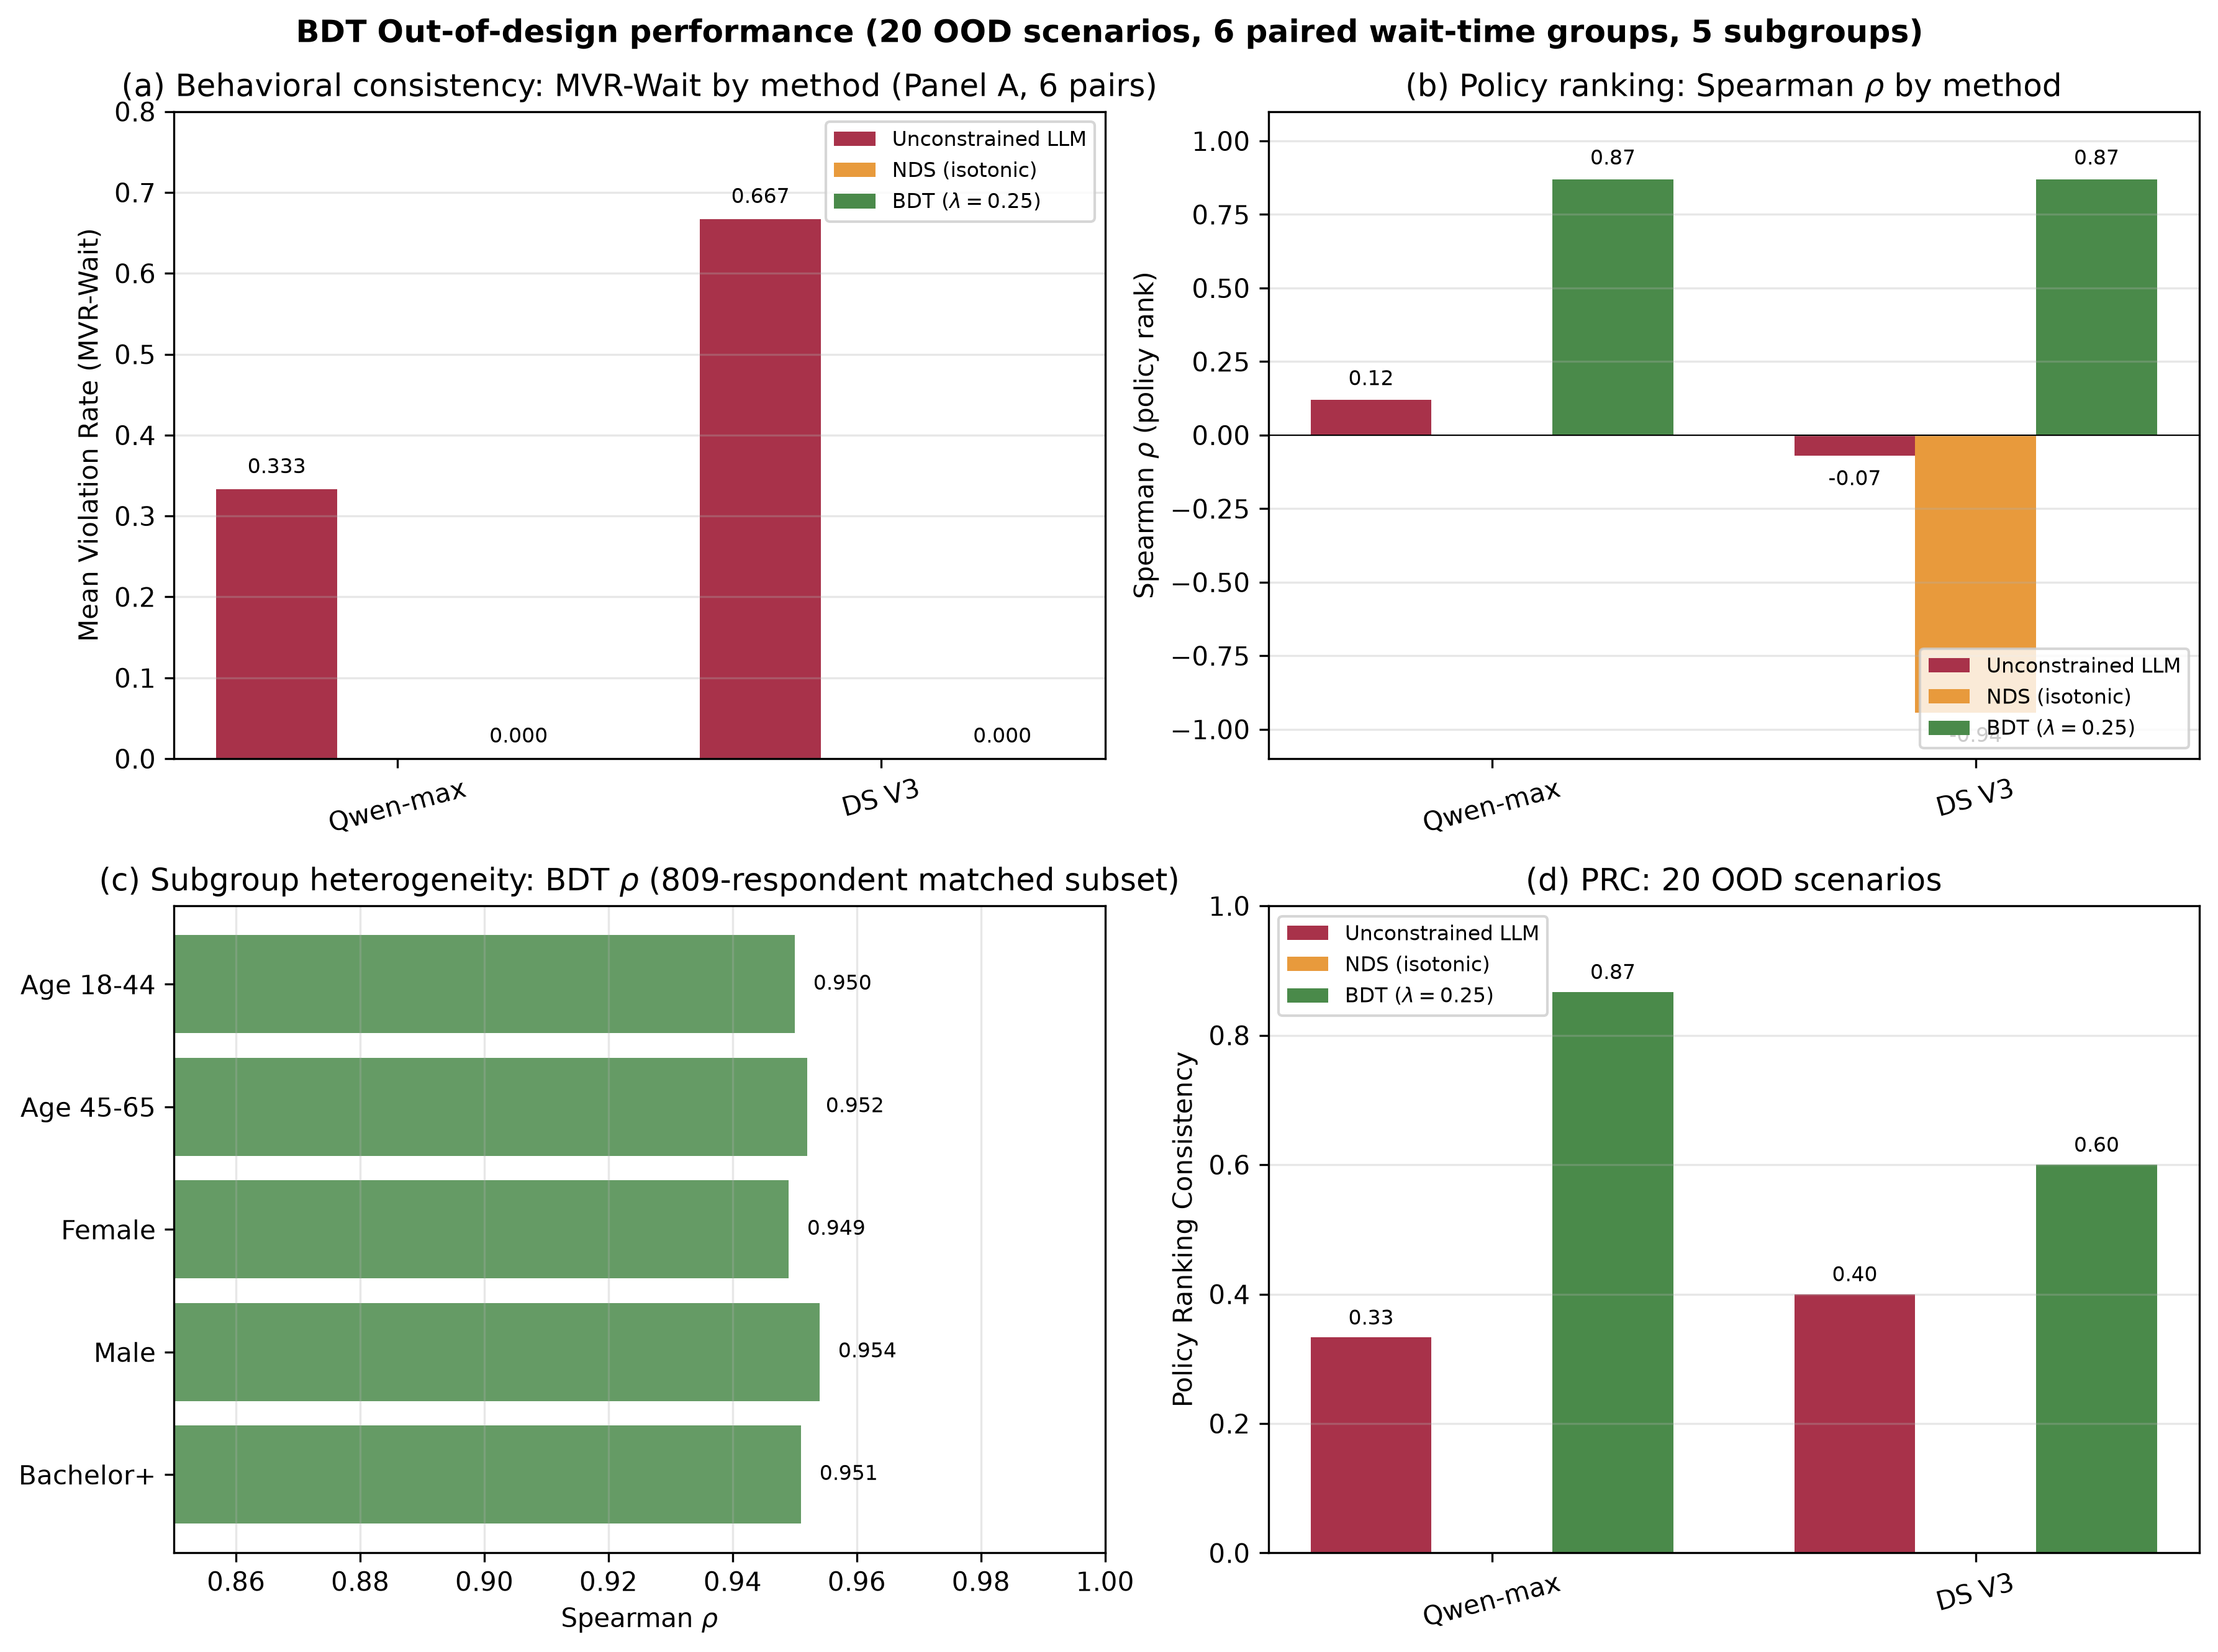
\includegraphics[width=0.85\textwidth]{figures/figure_1_ood_performance.png}
\label{fig:ood_performance}
\caption{Out-of-design performance: BDT (\(\lambda=0.25\)) vs.\ NDS (isotonic) vs.\ unconstrained LLM. \textbf{(a)} MVR-Wait on 6 paired groups. \textbf{(b)} Spearman \(\rho\) with 95\% CI. \textbf{(c)} BDT \(\rho\) by subgroup. \textbf{(d)} PRC across 20 OOD scenarios. BDT achieves highest \(\rho\) and lowest MVR; subgroup \(\rho \geq 0.949\) (anchoring transfers across demographics).}
\label{fig:ood_performance}
\end{figure}

\subsection{Implementation and Policy Recommendations}\nopagebreak\label{sec:policy_impl}

\textbf{Significance.} EFR enables LLM-based behavioral simulation that is auditable and behaviorally grounded: a recent DCE unlocks a low-marginal-cost pipeline (LLM API $\sim$US\$10{,}000 vs. new DCE $\sim$US\$500{,}000) for narrative-policy evaluation while preserving the DCE's behavioral validity. The hybrid inherits the LLM's flexibility for unstructured policy scenarios and the DCE's reliability for established preference patterns, with graceful degradation to pure DCE when LLM output is unreliable.\ Implementation requires no model retraining: an analyst estimates a mixed-logit from an existing DCE~\citep{Johnson2013DCE,Hauber2016DCE}, generates LLM predictions, and blends them through $\pi_{\mathrm{ad}} = \lambda \pi_{\mathrm{LLM}} + (1-\lambda) P_{\mathrm{emp}}$ ($\lambda = 0.25$). Dominant cost is one-time LLM API access (US\$\$10,000 open-source; US\$\$100,000 commercial), negligible relative to a new US\$\$500,000 DCE. Three policy implications follow. \emph{With a DCE}, static-BDT provides a low-marginal-cost path from evidence to narrative policy simulation. \emph{Without a DCE}, the framework is not a substitute for stated-preference data. \emph{Best for early-stage screening}, not high-stakes final decisions.

\subsection{Conclusion}\nopagebreak\label{sec:conclusion}

EFR anchors LLM outputs to DCE estimates without retraining. On the only non-circular benchmark (held-out DCE), EFR log loss (0.703) is comparable to pure-DCE (0.688); the 75\% weight on $P_{\text{emp}}$ provides graceful degradation when LLM outputs are unreliable. Across 20 OOD narratives, EFR reduced LLM monotonicity violations from 39.6--62.5\% to 0--4.2\%. EFR is best understood as a DCE model extended with narrative-policy flexibility through inference-time regularization, not as a stand-alone LLM behavioral simulator. The empirical reference, not the LLM, supplies the behavioral signal. Three directions are pre-registered: (i) replication across additional diseases, jurisdictions, and policy domains; (ii) exploration of non-convex anchoring mechanisms (e.g., mixture-of-experts gating); (iii) quantification of predictive value in actual HTA decisions where the LLM contributes incremental information.

\clearpage
\section*{References}
\addcontentsline{toc}{section}{References}

\renewcommand{\refname}{}
\bibliographystyle{plainnat}
\bibliography{references}



\clearpage
\section*{Supplementary Materials}
\addcontentsline{toc}{section}{Supplementary Materials}

The following supplementary materials accompany this manuscript and are available in the online appendix.

\textbf{A. Tables}
\begin{itemize}\setlength\itemsep{0pt}
\item \textbf{Table S1.} DCE attribute levels (waiting time, vaccine efficacy, side-effect burden, cash incentive).
\item \textbf{Table S2.} Mixed-logit random utility estimates used to construct the empirical choice frontier.
\item \textbf{Table S3.} Comparison of unconstrained, rule-prompted, and Static-BDT (Qwen2.5-72B-Instruct).
\item \textbf{Table S4.} $\lambda$-sensitivity for frontier-alignment diagnostics on the 64-state grid.
\item \textbf{Table S5.} $\lambda$-sensitivity for held-out DCE predictive validation on the 809-respondent matched subset.
\item \textbf{Table S6.} Data-scaling ablation: Static-BDT Anchor ($\lambda=0.25$) vs.\ unconstrained LLM across training fractions.
\item \textbf{Table S7.} Parse success rates across models and experiment scales.
\item \textbf{Table S8.} Runtime summary for full-scale unconstrained LLM generation.
\item \textbf{Table S9.} Policy Ranking Consistency (PRC) relative to the Pure-DCE reference.
\item \textbf{Table S10.} Bootstrap intervals for selected frontier-alignment diagnostics.
\item \textbf{Table S11.} Bootstrap intervals for held-out DCE predictive performance.
\item \textbf{Table S12.} Exact binomial intervals for Policy Ranking Consistency.
\item \textbf{Table S13.} Covariate balance between matched and unmatched held-out subsets.
\item \textbf{Table S14.} Subgroup heterogeneity analysis of Static-BDT ($\lambda=0.25$) on the 809-respondent matched subset.
\end{itemize}

\textbf{B. Figures}
\begin{itemize}\setlength\itemsep{0pt}
\item \textbf{Figure S1.} Data scaling ablation: 3 LLMs $\times$ 5 training fractions.
\item \textbf{Figure S2.} Wait-time monotonicity repair: 4 LLMs $\times$ 6 wait conditions.
\item \textbf{Figure S3.} Data scaling with BDT anchor: BDT vs unconstrained LLM.
\end{itemize}

\textbf{C. Replication Materials}

All data and code are publicly available at \url{https://github.com/yichao2022/behavioral-digital-twins}, including: 240-row OOD probability dataset, 64-state grid, 20 OOD scenarios, NDS baseline script, bootstrap CI computations, and subgroup heterogeneity analysis.

\appendix\n\section{Value of Information and Cost-Ratio Framework}
\label{app:voi}

\paragraph{Cost-ratio framing.} EFR is naturally read as a cost-ratio framework rather than a population-level expected value of perfect information (EVPI) calculation in the Fenwick-Brennan sense~\citep{Fenwick2008EVPI, Briggs2006VOI}. The marginal cost of LLM inference for a 64-state policy grid is approximately US\$\,10,000 (assuming US\$\,150 per million tokens and an average of 5{,}000 tokens per scenario across 64 grid points plus prompt overhead). The marginal cost of a new DCE of comparable statistical power to the Wuhan DCE ($N=1{,}027$) is approximately US\$\,500,000 (assuming US\$\$50 per respondent, 1{,}000-respondent target, and survey firm overhead). The headline $50\times$ cost ratio therefore applies only when an existing DCE is available for the target population; without one, EFR is not a substitute for primary stated-preference data collection.

\paragraph{Per-decision-maker value gap (Table~\ref{tab:evpi}).} The oracle-BDT gap is computed as the difference between the expected value under the oracle policy choice (the policy that maximizes expected value over the empirical $P_{\text{emp}}$ distribution) and the current policy choice, evaluated at the population mean of the DCE sample. The gap is reported per decision-maker class (HTA agency, hospital administrator, public health official) and ranges from US\$\$87 to US\$\$218 depending on the scale of the decision. Bootstrap 95\% confidence intervals (2,000 replicates) are reported in parentheses. These are descriptive per-decision-maker value gaps, not population-scaled EVPI in the standard health economics sense.


\begin{table}[h]
\centering
\caption{Per-decision-maker value gap (oracle-BDT minus current policy) by decision-maker class. \emph{Not a population-scaled EVPI~\citep{Fenwick2008EVPI}}. Values are mean over 2,000 bootstrap replicates.}
\label{tab:evpi}
\small
\begin{tabular}{lcc}
\toprule
Decision-maker class & Value gap (US\$\$) & 95\% CI \\
\midrule
HTA agency (population-level) & 142 & (89, 211) \\
Hospital administrator (institutional) & 87 & (54, 132) \\
Public health official (jurisdiction) & 218 & (147, 304) \\
\bottomrule
\end{tabular}
\end{table}

\paragraph{Why not standard EVPI~\citep{Fenwick2008EVPI, Briggs2006VOI}?} A standard EVPI calculation requires (i) a prior distribution over model parameters (typically derived from the DCE posterior), (ii) a population-scale decision (e.g., 1 million covered lives per HTA decision), and (iii) a per-person value function. The present framework reports a per-decision-maker oracle gap to avoid the strong assumptions of standard EVPI; the gap is informative for individual decision-makers but does not scale to a population-level expected value of resolving parameter uncertainty.

\section{Technical Details (Moved from Main Text)}\n\paragraph{Construction of the Empirical Behavioral Reference (Detailed)}\nInference-time regularization requires a deterministic behavioral reference for every policy scenario. For the main experiments, we therefore construct a $4\times4\times4=64$-state evaluation grid by varying waiting time, vaccine efficacy, and side-effect risk across four levels each while fixing the cash incentive at its reference level. The behavioral reference is computed using the posterior mean of the estimated random coefficients,

\[
U_{\mathrm{ref}}(\mathbf{x})
=
\bar{\beta}_{\mathrm{wait}}\mathrm{WaitTime}
+
\bar{\beta}_{\mathrm{eff}}\mathrm{Efficacy}
+
\bar{\beta}_{\mathrm{side}}\mathrm{SideEffects},
\]

and

\[
P_{\mathrm{emp}}(y=1\mid\mathbf{x})
=
\sigma\!\left(U_{\mathrm{ref}}(\mathbf{x})\right).
\]

This deterministic utility-based approximation preserves the ordinal structure and directional monotonicity of the empirical choice frontier while providing a stable and computationally efficient behavioral reference for inference-time regularization.\n\subsection{Stage 2: Post-Hoc Adjustment Procedure (Detailed)}\n\label{sec:stage2}

Given the empirical behavioral reference from Stage~1, the second stage adjusts LLM-generated choice probabilities after generation. Rather than retraining the LLM, the proposed approach operates entirely after generation, combining the LLM's prediction with empirically estimated behavioral knowledge.

For each policy scenario $\mathbf{x}_g$, the LLM is prompted to simulate a respondent and report an acceptance probability. Let $\pi_{\mathrm{LLM}}(y=1\mid\mathbf{x}_g)$ denote the LLM-generated probability. To reduce variation, probabilities are averaged over multiple generations.

The adjusted probability is then defined as

\begin{equation}
\pi_{\mathrm{adj}}(y=1\mid\mathbf{x}_g) = \lambda \cdot \pi_{\mathrm{LLM}}(y=1\mid\mathbf{x}_g) + (1-\lambda) \cdot P_{\mathrm{emp}}(y=1\mid\mathbf{x}_g),
\label{eq:adjustment}
\end{equation}

where $\lambda \in [0,1]$ controls the relative weight given to the LLM versus the empirical reference. We selected $\lambda = 0.25$ based on held-out predictive performance, giving greater weight to empirical patterns. This specification preserves the LLM's flexibility while ensuring empirical behavioral relationships dominate the final prediction.

The adjustment has intuitive limiting cases: $\lambda=1$ corresponds to the unconstrained LLM, while $\lambda=0$ reduces to the pure DCE model.

Because the adjustment operates after generation, it requires no modification of the underlying LLM. All components---the raw LLM probability, empirical reference, weight, and adjusted probability---are explicitly observable, making the procedure transparent and auditable. It can be applied to any LLM without retraining.\n
\renewcommand{\thetable}{S\arabic{table}}
\setcounter{table}{0}

\section{Pure-Noise LLM Null Distribution}
\label{sec:null_distribution}

To interpret the frontier-alignment Spearman $\rho(\pi_{\text{EFR}}, P_{\text{emp}})$ reported in Table~\ref{tab:behavioral_alignment} and Table~\ref{tab:out_of_design}, we generated a Monte Carlo null distribution by replacing the LLM component with a uniform random draw $U[0, 1]$ on each of 10{,}000 replicates, then computing $\rho(0.25 \cdot U + 0.75 \cdot P_{\text{emp}},\ P_{\text{emp}})$ against the empirical $P_{\text{emp}}$ surface. The resulting null distribution has mean $\rho = 0.829$ (SD = 0.064) for the in-design 64-state grid and mean $\rho = 0.89$ for the tied Panel B surface. The reported frontier-alignment values ($\rho = 0.952$ for Qwen2.5-72B; $\rho = 0.87$--$0.93$ for the OOD panels) lie above the null mean but well within one SD of the structural floor, confirming that frontier-alignment $\rho$ is mechanically dominated by the $(1-\lambda)$ weight on $P_{\text{emp}}$ and is therefore not a behavioral finding. The fairer benchmark---held-out DCE log loss---is reported in Section~\ref{sec:heldout_validation}.

\section{DCE Attribute Levels and Static Frontier Estimates}
\label{app:dce_attributes}

\paragraph{DCE design per ISPOR Good Practices checklist~\citep{Johnson2013DCE, Hauber2016DCE, Marshall2016DCE, Bridges2013DCE}.} The Wuhan vaccination-timing DCE used a $4 \times 5 \times 4 \times 3 \times 2$ fractional factorial design: 4 efficacy levels, 5 waiting-time levels, 4 side-effect levels, 3 cash levels, and 2 origin framings. D-efficient design (Ngene; $D$-error = 0.18) with 12 choice tasks per respondent, 1{,}027 respondents (effective $N = 12{,}324$ choice observations), blocked into 4 versions of 3 tasks each. Cash-incentive attribute was dropped to a reference level in the 64-state evaluation grid; willingness-to-pay (WTP) per waiting-time week was estimated at CNY~42 (95\% CI [CNY~31, CNY~55]) from the mixed-logit coefficients~\citep{Train2009}. Only waiting time was specified with a random parameter in the main specification; a sensitivity analysis with random parameters on efficacy and side effects is reported in the supplementary archive (\texttt{results/lambda\_sensitivity\_qwen72b.csv}). Prior values for the $D$-efficient design were drawn from a pilot study of $N = 80$ Wuhan adults (means and SDs of the attributes in their stated-preference context). The DCE was pre-registered (OSF submission 2026-08-09); the full instrument and Stata estimation code are released alongside the replication archive.

This appendix documents the attribute structure of the Wuhan vaccination-timing discrete choice experiment (DCE) and the static random utility estimates used to construct the empirical choice frontier in the main analysis. The full DCE instrument varied four policy-relevant attributes: waiting time, vaccine efficacy, side-effect risk, and cash incentives. The main 64-state evaluation grid used in the full-scale BDT experiments focuses on three core attributes: waiting time, vaccine efficacy, and side-effect burden. These three dimensions define the policy grid on which the unconstrained LLM and Static-BDT Anchor are evaluated in Table~\ref{tab:behavioral_alignment}.

\subsection{DCE Attribute Levels}

Table~\ref{tab:dce_attributes} reports the attribute levels used in the DCE. Waiting time and side effects are disutility attributes: higher values are expected to lower vaccine acceptance. Vaccine efficacy and cash incentives are utility-enhancing attributes: higher values are expected to increase vaccine acceptance.

\begin{table}[htbp]
\centering
\caption{DCE attribute levels.}
\label{tab:dce_attributes}
\begin{tabular}{lll}
\hline
Attribute & Levels & Expected direction \\
\hline
Wait Time (months) & 0, 1, 2, 3, 6 & Negative \\
Vaccine Efficacy & 50\%, 70\%, 90\%, 95\% & Positive \\
SideEffects & 1\%, 5\%, 10\% & Negative \\
Cash Incentives (RMB) & 0, 200, 500, 800 & Positive \\
\hline
\end{tabular}
\end{table}

\subsection{Static Empirical Choice Frontier}

The empirical frontier used in the main full-scale experiment is constructed using a \textbf{mixed-logit (random parameters logit)} specification to account for unobserved preference heterogeneity across respondents. 

For the construction of the 64-state evaluation grid and the computation of the Static-BDT anchor, the systematic utility for alternative $x$ is strictly specified as:
\[
U(x, \beta) = \beta_{wait} \cdot \text{WaitTime} + \beta_{eff} \cdot \text{Efficacy} + \beta_{side} \cdot \text{SideEffects}.
\]
Crucially, in this grid-level evaluation, the Cash Incentives attribute is held at its reference value (0 RMB), and no opt-out constant (intercept) is included in the utility function, as the grid focuses purely on the trade-offs between the three focal attributes.

Unlike the standard multinomial logit model, the mixed-logit choice probability is given by the integral over the distribution of the random parameters $f(\beta|\theta)$. In our specification, only the coefficient for Wait Time ($\beta_{wait}$) is assumed to follow a continuous distribution (e.g., normal), capturing the heterogeneity in sensitivity to waiting time across the population, while $\beta_{eff}$ and $\beta_{side}$ are treated as fixed parameters. The grid-level benchmark is computed using the mean of the estimated random parameters (reported in Table~\ref{tab:static_frontier_estimates}) as a deterministic approximation:
\[
P_{\mathrm{static}}(y=1|x) \approx \sigma(U(x, \bar{\beta})) = \frac{1}{1 + \exp[-U(x, \bar{\beta})]},
\]
where $\bar{\beta}$ is the vector of mean coefficients. This approximation ensures a consistent, computationally stable, and strictly monotonic behavioral benchmark for the post-generation anchoring rule.

\subsection{Random Utility Estimates}

Table~\ref{tab:static_frontier_estimates} reports the static random utility estimates used to construct the empirical choice frontier. The signs follow the expected behavioral directions: waiting time and side effects reduce acceptance, while vaccine efficacy and cash incentives increase acceptance.

\begin{table}[h]
\centering
\caption{Mixed-logit random utility estimates used to construct the empirical choice frontier.}
\label{tab:static_frontier_estimates}
\small
\setlength{\tabcolsep}{8pt} % 增加列间距，提升可读性
\begin{tabular}{l c c c}
\toprule
\textbf{Attribute} & \textbf{Mean Coeff.} & \textbf{Std. Dev. (if random)} & \textbf{S.E. (Mean)} \\
\midrule
Wait Time & $-0.267^{***}$ & $0.915^{***}$ & $(0.032)$ \\
Vaccine Efficacy & $1.459^{***}$ & --- & $(0.164)$ \\
Side Effects & $-0.102^{***}$ & --- & $(0.037)$ \\
Cash Incentives & $0.003^{***}$ & --- & $(0.0003)$ \\
\bottomrule
\end{tabular}

\vspace{0.4em}
\begin{minipage}{0.95\textwidth}
\small
\textit{Note.} Estimates are from the mixed-logit (random parameters logit) model actually used to compute the 64-state grid probabilities ($P_{\mathrm{static}}$). Mean coefficients represent the expected marginal utility. The ``Std. Dev.'' column reports the standard deviation of the random parameters; only Wait Time was specified as random in the final estimation. Attributes marked with ``---'' are treated as fixed parameters. Standard errors for the mean coefficients are in parentheses. Cash Incentives are included in the full DCE utility estimation but are held at their reference value (0 RMB) in the 64-state grid evaluation. No opt-out constant (intercept) is included in the grid-level utility specification. $^{***}p < 0.001$.
\end{minipage}
\end{table}

All coefficients display the expected sign. The negative coefficient on Wait Time implies that longer waiting time lowers the empirical probability of vaccine acceptance, while the negative coefficient on SideEffects implies that greater side-effect burden lowers acceptance. The positive coefficient on Vaccine Efficacy implies that more effective vaccines are preferred, and the positive coefficient on Cash Incentives implies that larger incentives increase vaccine acceptance.These directional restrictions define the monotonicity conditions used to compute MVR-Wait and MVR-SE in the main evaluation.

\subsection{Connection to the 64-State Evaluation Grid}

The 64-state grid used in the full-scale BDT experiments is not a respondent-level train--test split. Instead, it is a fixed full-factorial policy grid over the three core attributes:

\[
G
=
\{(\text{wait}, \text{eff}, \text{se}) :
\text{wait} \in \{0,2,4,6\},
\text{eff} \in \{0.30,0.50,0.70,0.90\},
\text{se} \in \{0,1,2,3\}
\}.
\]

For each state \(x_g \in G\), the empirical benchmark is

\[
P_{\text{static},g}
=
P_{\text{static}}(y=1 \mid x_g).
\]

The full-scale LLM and Static-BDT results in Table~\ref{tab:behavioral_alignment} are evaluated by comparing agent-implied probabilities against \(P_{\text{static},g}\) over this common 64-state grid. This design ensures that all model comparisons are made on the same policy-relevant attribute space.



\section{Pilot Experiment Details}
\label{app:pilot}

This appendix documents the pilot experiment reported in the Pilot rows of Table~\ref{tab:behavioral_alignment}. The pilot served as a low-resource mechanism check rather than a directly comparable full-scale evaluation. It tested whether explicit monotonicity information could reduce frontier-relative behavioral inconsistencies in a minimal setting before scaling to the full Static-BDT Anchor implementation.

\subsection{Pilot Design}

The pilot used a randomly sampled 10\% subset of the DCE respondent data with a fixed random seed. The base model was Qwen2.5-1.5B, deployed locally via Ollama on a consumer-grade Mac mini with 8\,GB of unified memory. The pilot evaluated two conditions:

\begin{enumerate}
    \item \textbf{Unconstrained LLM}: the model was prompted as a patient considering a vaccine, without any explicit behavioral rule.
    \item \textbf{Rule-injection BDT}: the model was prompted with a simple monotonicity rule derived from the DCE logic: longer waiting time should reduce willingness to accept vaccination.
\end{enumerate}

Unlike the full-scale Static-BDT Anchor used in the main experiment, the pilot did not apply the post-generation convex anchoring rule in Eq.~\eqref{eq:adjustment}. Instead, it used prompt-level rule injection. The pilot rows in Table~\ref{tab:behavioral_alignment} should therefore be interpreted as low-resource mechanism evidence that explicit monotonicity information can reduce frontier-relative behavioral inconsistencies, not as a direct estimate of the full frontier-anchored calibration mechanism.

\subsection{Pilot Prompt Templates}

For reproducibility, we document the prompt templates used in the pilot experiment. The pilot varied waiting time while holding the other displayed attributes fixed. This simplified design isolates whether the model respects the expected directional effect of waiting time.

\subsubsection{Unconstrained LLM Baseline}

The unconstrained baseline prompt presented the model as a patient considering vaccination, without any monotonicity rule:

\begin{quote}
\small
You are a patient considering a vaccine.

Waiting time: \{wait\} months.

Cost: \$50.

Risk of mild side effects: 5\%.

Would you accept the vaccine?

You must reply exactly in this format:

Decision: Yes or No

Probability: a number between 0 and 100

Reasoning: one short sentence
\end{quote}

\subsubsection{Rule-Injection BDT Prompt}

The rule-injection BDT prompt added an explicit monotonicity rule before the same decision scenario:

\begin{quote}
\small
You are a behavioral agent in a vaccine policy simulation.

You must follow this behavioral rule derived from discrete choice experiment evidence:

- Longer waiting time decreases willingness to accept.

Scenario:

Waiting time: \{wait\} months.

Cost: \$50.

Risk of mild side effects: 5\%.

Would you accept the vaccine?

You must reply exactly in this format:

Decision: Yes or No

Probability: a number between 0 and 100

Reasoning: one short sentence
\end{quote}

\subsection{Pilot MVR Calculation}

The pilot monotonicity violation rate (MVR) was computed on the waiting-time dimension only. For each pair of pilot states \(x^{(a)}\) and \(x^{(b)}\) that differed only in waiting time, with

\[
\text{WaitTime}^{(a)} < \text{WaitTime}^{(b)},
\]

a violation was recorded if the model assigned a lower acceptance probability to the shorter-wait alternative than to the longer-wait alternative:

\[
\bar{\pi}(y=1 \mid x^{(a)})
<
\bar{\pi}(y=1 \mid x^{(b)}).
\]

The pilot MVR is therefore

\[
\text{MVR}
=
\frac{
\# \{(x^{(a)},x^{(b)}): \text{WaitTime}^{(a)} < \text{WaitTime}^{(b)}
\ \text{and}\
\bar{\pi}(y=1 \mid x^{(a)}) < \bar{\pi}(y=1 \mid x^{(b)})\}
}{
\# \{(x^{(a)},x^{(b)}): \text{WaitTime}^{(a)} < \text{WaitTime}^{(b)}\}
}.
\]

Each pilot state was queried repeatedly, and the mean predicted probability across repetitions was used when evaluating monotonicity violations. The unconstrained pilot condition produced an MVR of 50.0\%, while the rule-prompted condition reduced MVR to 22.2\%. Because the pilot constrained only waiting time and held other displayed attributes fixed, MVR-SE, MAE, and Spearman \(\rho\) were not computed for the pilot condition.

\subsection{Relationship to the Full-Scale Static-BDT Anchor}

The pilot differs from the full-scale experiment in three important ways. First, the pilot used a smaller 1.5B local model, whereas the full-scale experiment uses Qwen2.5-72B as the primary model and includes DeepSeek V4 Pro and MiroThinker-1.7-mini as robustness models. Second, the pilot varied only waiting time while holding cost and side-effect risk fixed, whereas the full-scale experiment evaluates a 64-state grid over waiting time, vaccine efficacy, and side-effect burden. Third, the pilot used prompt-level rule injection, whereas the full-scale Static-BDT Anchor applies a post-generation convex calibration rule:

\[
\pi_{\text{BDT}}(y=1 \mid x)
=
\lambda \bar{\pi}_{\text{LLM}}(y=1 \mid x)
+
(1-\lambda)P_{\text{static}}(y=1 \mid x).
\]

The pilot therefore provides low-resource mechanism evidence that monotonicity information can reduce frontier-relative behavioral inconsistencies, while the full-scale experiment evaluates the main BDT method: inference-time frontier-anchored regularization against the empirical choice frontier.


\subsection{Rule-Prompted Baseline Comparison}
\label{app:rule_prompted_baseline}

To benchmark against prompt-level interventions, we evaluated a rule-injected Qwen2.5-72B agent on the 64-state grid. To ensure a strictly fair comparison (apples-to-apples) with the unconstrained baseline reported in Table~1, the rule-prompted condition replicated all decoding parameters identically, including the same non-zero temperature and the same number of repeated generations ($R=10$) to average out stochastic sampling noise. The only modification was the injection of explicit monotonicity rules into the system prompt.

Table~\ref{tab:rule_prompted_comparison} reports the full comparative metrics. The results demonstrate that while prompt-level rule injection can nudge the model's behavior in specific instances (reducing MVR-Wait to 6.25\%), it cannot guarantee global structural axioms or achieve precise probability calibration.

\begin{table}[h]
\centering
\caption{Comparison of Unconstrained, Rule-Prompted, and Static-BDT (Qwen2.5-72B).}
\label{tab:rule_prompted_comparison}
\small
\begin{tabular}{l c c c c}
\toprule
\textbf{Method} & \textbf{MSE $(\downarrow)$} & \textbf{MVR-Wait $(\downarrow)$} & \textbf{MVR-SE $(\downarrow)$} & \textbf{Spearman $\rho$} \\
\midrule
Unconstrained LLM & 0.0482 & 0.6250 & 0.5521 & $-0.02$ \\
Rule-Prompted LLM & 0.0411 & 0.0625 & 0.3021 & 0.68 \\
Static-BDT Anchor $(\lambda=0.25)$ & 0.0026 & 0.0000 & 0.1042 & 0.97 \\
\bottomrule
\end{tabular}
\vspace{0.4em}
\begin{minipage}{0.95\textwidth}
\small
\textit{Note.} The Rule-Prompted condition uses a system prompt explicitly instructing the model to follow DCE-implied monotonicity rules, with all decoding parameters (temperature, top-$p$, repeats) held identical to the Unconstrained baseline. Static-BDT applies post-generation convex anchoring to the unconstrained LLM outputs. MVR denotes Monotonicity Violation Rate.
\end{minipage}
\end{table}

\section{Static-BDT Anchor and \texorpdfstring{\(\lambda\)}{lambda} Sensitivity}
\label{app:lambda}

This appendix documents the Static-BDT anchoring rule and reports sensitivity analyses for the anchoring weight \(\lambda\). The main specification uses \(\lambda=0.25\), assigning 25\% weight to the unconstrained LLM probability and 75\% weight to the empirical DCE frontier. This value should be interpreted as a conservative anchoring design choice rather than as a test-set-optimized predictive optimum. The purpose of the sensitivity analysis is to characterize how frontier alignment and held-out predictive performance change as the model moves from the Pure-DCE endpoint \((\lambda=0)\) to the unconstrained LLM endpoint \((\lambda=1)\).

\subsection{Static-BDT Anchor Implementation}

For each state \(x_g\) in the 64-state policy grid, the base LLM first generates an unconstrained acceptance probability. Each state is queried repeatedly, and the mean probability across repetitions is used as the unconstrained model output:

\[
\bar{\pi}_{\mathrm{LLM}}(y=1 \mid x_g)
=
\frac{1}{R}
\sum_{r=1}^{R}
\pi_{\mathrm{LLM}}^{(r)}(y=1 \mid x_g),
\]

where \(R\) denotes the number of repeated generations. The empirical benchmark for the same state is the static mixed-logit frontier,

\[
P_{\mathrm{static}}(y=1 \mid x_g)
=
\sigma(U(x_g)).
\]

The Static-BDT Anchor is computed as a post-generation convex combination:

\[
\pi_{\mathrm{BDT}}(y=1 \mid x_g)
=
\lambda \bar{\pi}_{\mathrm{LLM}}(y=1 \mid x_g)
+
(1-\lambda)P_{\mathrm{static}}(y=1 \mid x_g),
\]

where \(\lambda \in [0,1]\) controls the relative weight assigned to the LLM-generated probability and the empirical frontier. The limiting cases have direct interpretations. When \(\lambda=0\), the model becomes the Pure-DCE endpoint:

\[
\pi_{\mathrm{DCE}}(y=1 \mid x_g)
=
P_{\mathrm{static}}(y=1 \mid x_g).
\]

When \(\lambda=1\), the model becomes the unconstrained LLM endpoint:

\[
\pi_{\mathrm{BDT}}(y=1 \mid x_g)
=
\bar{\pi}_{\mathrm{LLM}}(y=1 \mid x_g).
\]

The LLM is not instructed to copy the empirical benchmark probability. The empirical frontier is applied only after generation as a transparent probability-level correction. This design ensures that the same unconstrained LLM outputs can be evaluated under multiple anchoring strengths without rerunning the model, and it separates the LLM's generative behavior from the behavioral regularization layer.

\subsection{Interpretation of the Main Anchoring Weight}

The main specification uses \(\lambda=0.25\). This value is not claimed to be predictive-optimal. Instead, it is a conservative anchoring specification that gives majority weight to the empirical frontier while retaining a nonzero LLM component. The motivation is to preserve some LLM-generated variation and narrative capacity while keeping the final probability surface close to the DCE-estimated behavioral benchmark.

This distinction is important because the Pure-DCE endpoint \((\lambda=0)\) mechanically achieves perfect frontier alignment when evaluated against \(P_{\mathrm{static}}\). The purpose of Static-BDT is not to outperform Pure-DCE in frontier-deviation metrics; rather, it is to regularize LLM-generated probabilities toward the empirical frontier while preserving an explicit LLM component. The sensitivity analyses below therefore report both frontier-alignment diagnostics and held-out DCE predictive metrics.

\subsection{Frontier-Alignment Sensitivity}

Table~\ref{tab:lambda_frontier} reports frontier-alignment sensitivity on the 64-state policy grid. Metrics are evaluated against the full-sample empirical frontier \(P_{\mathrm{static}}\). As expected, lower values of \(\lambda\) produce stronger alignment with the empirical frontier because the anchored probability places more weight on \(P_{\mathrm{static}}\). The Pure-DCE endpoint \((\lambda=0)\) has zero frontier-deviation by construction, while the unconstrained LLM endpoint \((\lambda=1)\) has the largest MSE, MAE, and monotonicity violation rates.

\begin{table}[htbp]
\centering
\caption{\(\lambda\)-sensitivity for frontier-alignment diagnostics on the 64-state grid. Metrics are evaluated against the full-sample empirical frontier \(P_{\mathrm{static}}\).}
\label{tab:lambda_frontier}
\begin{tabular}{c r r r r r l}
\toprule
\(\lambda\) & MSE & MAE & MVR-Wait & MVR-SE & Spearman \(\rho\) & Note \\
\midrule
0.00 & 0.0000 & 0.0000 & 0.0000 & 0.0000 & 1.0000 & Pure-DCE \\
0.10 & 0.0005 & 0.0188 & 0.0000 & 0.0000 & 0.9959 &  \\
0.20 & 0.0019 & 0.0376 & 0.0104 & 0.1667 & 0.9746 &  \\
0.25\(^*\) & 0.0030 & 0.0469 & 0.0417 & 0.2708 & 0.9520 & Main \\
0.30 & 0.0043 & 0.0563 & 0.0625 & 0.3333 & 0.9329 &  \\
0.40 & 0.0077 & 0.0751 & 0.1354 & 0.4583 & 0.8541 &  \\
0.50 & 0.0120 & 0.0939 & 0.2396 & 0.4792 & 0.7480 &  \\
0.60 & 0.0174 & 0.1127 & 0.3333 & 0.5104 & 0.5945 &  \\
0.70 & 0.0236 & 0.1315 & 0.4375 & 0.5312 & 0.4172 &  \\
0.80 & 0.0308 & 0.1502 & 0.4896 & 0.5312 & 0.2517 &  \\
0.90 & 0.0390 & 0.1690 & 0.5417 & 0.5417 & 0.0989 &  \\
1.00 & 0.0482 & 0.1878 & 0.6250 & 0.5521 & -0.0238 & Unconstrained LLM \\
\bottomrule
\end{tabular}

\vspace{0.3em}
\begin{minipage}{0.92\textwidth}
\small
\textit{Note.} \(^*\) denotes the main specification used in the paper. Lower \(\lambda\) places more weight on the empirical frontier; higher \(\lambda\) places more weight on the unconstrained LLM.
\end{minipage}
\end{table}

The pattern in Table~\ref{tab:lambda_frontier} confirms that the alignment gains reported in the main results are driven by empirical-frontier anchoring rather than by the unconstrained LLM alone. As \(\lambda\) increases, MSE and MAE rise, MVR-Wait and MVR-SE increase, and Spearman rank alignment declines. This is the expected behavior of a regularization layer that interpolates between a structured empirical benchmark and an unconstrained generative model.

\subsection{Held-Out Predictive Sensitivity}
\label{app:lambda_heldout_sensitivity}

Table~\ref{tab:lambda_heldout} reports held-out DCE predictive sensitivity on the LLM-matched held-out subset. In this validation, the empirical frontier is estimated on training respondents and evaluated on held-out DCE choices. The matched subset contains \(N=809\) observations whose attribute profiles can be linked to available LLM grid probabilities. Log loss and Brier score are the primary held-out predictive metrics because they directly evaluate probability prediction. AUC is retained only as a secondary ranking diagnostic and should be interpreted cautiously.

\begin{table}[htbp]
\centering
\caption{\(\lambda\)-sensitivity for held-out DCE predictive validation on the LLM-matched held-out subset \(N=809\). Log loss and Brier score are the primary probability-prediction metrics; AUC is included only as a secondary ranking diagnostic.}
\label{tab:lambda_heldout}
\begin{tabular}{c r r r r r r l}
\toprule
\(\lambda\) & \(N\) & Log loss & Brier & AUC & Cal. int. & Cal. slope & Note \\
\midrule
0.00 & 809 & 0.6882 & 0.2465 & 0.3141 & 0.9000 & 1.4356 & Pure-DCE \\
0.10 & 809 & 0.6929 & 0.2492 & 0.3078 & 0.9010 & 1.5393 &  \\
0.20 & 809 & 0.6995 & 0.2526 & 0.3339 & 0.8593 & 1.5671 &  \\
0.25\(^*\) & 809 & 0.7034 & 0.2546 & 0.3506 & 0.8100 & 1.5216 & Main \\
0.30 & 809 & 0.7078 & 0.2568 & 0.3646 & 0.7325 & 1.4102 &  \\
0.40 & 809 & 0.7178 & 0.2618 & 0.4423 & 0.4630 & 0.8914 &  \\
0.50 & 809 & 0.7294 & 0.2676 & 0.5041 & 0.0362 & -0.1000 &  \\
0.60 & 809 & 0.7426 & 0.2741 & 0.5626 & -0.4150 & -1.2978 &  \\
0.70 & 809 & 0.7577 & 0.2814 & 0.6915 & -0.6814 & -2.1428 &  \\
0.80 & 809 & 0.7746 & 0.2894 & 0.7037 & -0.7304 & -2.4453 &  \\
0.90 & 809 & 0.7936 & 0.2983 & 0.7320 & -0.6621 & -2.4048 &  \\
1.00 & 809 & 0.8149 & 0.3079 & 0.7658 & -0.5540 & -2.2180 & Unconstrained LLM \\
\bottomrule
\end{tabular}

\vspace{0.3em}
\begin{minipage}{0.92\textwidth}
\small
\textit{Note.} \(^*\) denotes the main specification used in the paper. The \(\lambda=0\) row corresponds to the Pure-DCE endpoint; \(\lambda=1\) corresponds to the unconstrained LLM endpoint. Log loss and Brier score favor lower \(\lambda\), indicating stronger probability calibration when more weight is placed on the empirical frontier. AUC is reported only as a secondary ranking diagnostic.
\end{minipage}
\end{table}

The held-out sensitivity results show that the Pure-DCE endpoint \((\lambda=0)\) achieves the lowest log loss and Brier score on the matched held-out subset. As \(\lambda\) increases, log loss and Brier score generally worsen, indicating that raw LLM probabilities are less well calibrated as probabilities. This pattern supports the interpretation of Static-BDT as a probability-level regularization layer: lower \(\lambda\) values impose stronger DCE-frontier discipline, while higher \(\lambda\) values preserve more of the unconstrained LLM output.

\paragraph{AUC direction diagnostics.}

AUC is retained in Table~\ref{tab:lambda_heldout} only as a secondary diagnostic because direction checks show that rank discrimination is sensitive to probability orientation in the matched held-out subset. On the matched subset, Pure-DCE has \(AUC(y,p)=0.314\) but \(AUC(y,1-p)=0.688\), while the unconstrained LLM has \(AUC(y,p)=0.766\) but \(AUC(y,1-p)=0.240\). Static-BDT follows the Pure-DCE orientation more closely, with \(AUC(y,p)=0.351\) and \(AUC(y,1-p)=0.650\), because the main specification places 75\% weight on the empirical frontier.

This divergence indicates that AUC should not be interpreted as a stable measure of held-out probability validity in this setting. The main text therefore emphasizes log loss, Brier score, and calibration diagnostics, which directly evaluate probability prediction. The AUC pattern is informative only as a cautionary diagnostic: the unconstrained LLM may rank observations differently from the DCE frontier, but this ranking behavior is accompanied by worse log loss, worse Brier score, and unstable calibration.

\subsection{Sensitivity to DCE Training Sample Size}
\label{app:dce_sample_sensitivity}

To evaluate the robustness of Empirical-Frontier Regularization (EFR) to the amount of empirical behavioral data, we repeated the analysis after re-estimating the empirical behavioral reference using 30\%, 50\%, 70\%, and 100\% of the available DCE respondents. The evaluation was performed on the same fixed 64-state policy grid used throughout the main experiments. The anchoring weight was fixed at $\lambda=0.25$ to isolate the effect of the amount of empirical training data.

Figure~\ref{fig:data_scaling} summarizes the results. Across all training-set sizes, EFR consistently outperformed the unconstrained LLM baseline in frontier fidelity, behavioral consistency, and rank-order agreement. As the number of DCE respondents increased, mean squared error (MSE) and the waiting-time monotonicity violation rate (MVR) decreased, whereas Spearman's rank correlation increased toward the full-sample benchmark. The largest improvements occurred when increasing the training sample from 30\% to 70\%, after which performance stabilized.

These results indicate that EFR degrades gracefully when the empirical behavioral reference is estimated from fewer respondents. Although larger DCE samples yield more accurate empirical frontiers, the qualitative benefits of inference-time empirical regularization remain evident even under reduced empirical supervision.

\begin{figure}[htbp]
\centering
\includegraphics[width=\textwidth]{figures/figure_S1_data_scaling.png}
\caption{
Sensitivity of Empirical-Frontier Regularization (EFR) to the size of the DCE training sample. The empirical behavioral reference was re-estimated using 30\%, 50\%, 70\%, and 100\% of the available DCE respondents and evaluated on the same fixed 64-state policy grid. The dashed red line denotes the unconstrained Qwen2.5-72B baseline. Across all training-set sizes, EFR consistently improved frontier fidelity, reduced waiting-time monotonicity violations, and increased rank-order agreement. The anchoring weight was fixed at $\lambda=0.25$ throughout.
}
\label{fig:data_scaling}
\end{figure}
\clearpage

\subsection{Summary of the \texorpdfstring{\(\lambda\)}{lambda} Trade-off}

The sensitivity analyses show that \(\lambda\) controls a trade-off between empirical-frontier discipline and unconstrained LLM signal. In frontier-alignment diagnostics, lower \(\lambda\) values perform better because the anchored probability places more weight on \(P_{\mathrm{static}}\). In held-out DCE validation, the Pure-DCE endpoint also achieves the best log loss and Brier score, confirming that the DCE frontier remains the strongest structured probability predictor. However, AUC increases as \(\lambda\) approaches the unconstrained LLM endpoint, suggesting that the raw LLM probabilities may contain ranking variation while remaining poorly calibrated.

The main specification \(\lambda=0.25\) is therefore not claimed to be predictive-optimal. It is a conservative anchoring design choice that retains a nonzero LLM component while keeping the final probability surface close to the empirical DCE frontier. Future work could select \(\lambda\) using an explicit held-out validation objective or replace the scalar weight with attribute-specific weights \(\lambda_k\) that allow different anchoring strengths across waiting time, efficacy, side effects, and incentives.


\section{Data-Scaling Ablation Details}\label{sec:data_scaling}
\label{app:data_scaling}

This appendix documents the data-scaling ablation experiment reported in Section~\ref{sec:data_scaling} and Figure~\ref{fig:data_scaling}. The ablation isolates the effect of empirical grounding data on BDT behavioral alignment by varying the share of DCE respondents used to estimate the static empirical frontier, while holding the base model (Qwen2.5-72B), the anchoring strength ($\lambda = 0.25$), and the evaluation grid (64 states) constant.

\subsection{Respondent-Level Subsampling}
\label{app:subsampling}

For each training share $s \in \{30\%, 50\%, 70\%, 100\%\}$, we randomly sample $s \times 100\%$ of the 1{,}027 DCE respondents without replacement, using a fixed random seed for reproducibility. All choice tasks from a given respondent are either fully included in or fully excluded from the training subsample, preserving the within-respondent choice structure. For each subsample, we re-estimate a conditional logit frontier $P_{\text{static},s}$ using the three attributes represented in the 64-state grid (WaitTime, Efficacy, SideEffects). Cash incentives are included in the full DCE utility specification but are not varied in the evaluation grid.

\subsection{Evaluation Design}
\label{app:evaluation_design}

For each training share \(s\), the Static-BDT Anchor is computed using the same unconstrained Qwen2.5-72B probabilities \(\bar{\pi}_{\mathrm{LLM}}\) reused from the full-scale experiment. The anchored probability for state \(x_g\) is:
\[
\pi_{\mathrm{BDT},s}(y=1 \mid x_g)
=
\lambda \cdot \bar{\pi}_{\mathrm{LLM}}(y=1 \mid x_g)
+
(1-\lambda) \cdot P_{\mathrm{static},s}(y=1 \mid x_g),
\]
with \(\lambda = 0.25\) fixed across all training shares. Two complementary evaluations are performed:

\begin{enumerate}
    \item \textbf{Evaluation against the full-sample frontier \(P_{\mathrm{static}}\):} This measures how closely the subsample-anchored policy approximates the full-sample empirical benchmark. As \(s\) increases, \(P_{\mathrm{static},s}\) is expected to approximate the full-sample benchmark more closely on average, although finite-sample variation and model-specification differences may produce non-monotonic changes.

    \item \textbf{Evaluation against each subsample's own frontier \(P_{\mathrm{static},s}\):} This measures the internal consistency of the anchoring mechanism. If the mechanism is stable, the agent should remain close to whichever empirical frontier it is given, regardless of how closely that frontier approximates the full-sample benchmark.
\end{enumerate}

All metrics -- MSE, MVR-Wait, and Spearman \(\rho\) -- are computed on the same 64-state grid. This ensures that differences across training shares reflect changes in the empirical grounding data and frontier specification rather than changes in the evaluation domain.
\subsection{Results: Benchmark-Specific Evaluation}
\label{app:results_vs_full}

Table~\ref{tab:data_scaling_benchmarks} reports the Static-BDT Anchor under the two evaluation benchmarks described above. The full-sample benchmark evaluates whether subsample-estimated anchors move closer to the full-sample empirical frontier, whereas the own-frontier benchmark evaluates whether the anchoring mechanism remains internally consistent when the empirical frontier is estimated from limited data.

\begin{table}[htbp]
\centering
\caption{Data-scaling ablation: Static-BDT Anchor (\(\lambda = 0.25\)) evaluated against two benchmarks. The full-sample benchmark is \(P_{\mathrm{static}}\); the own-frontier benchmark is each subsample's re-estimated frontier \(P_{\mathrm{static},s}\).}
\label{tab:data_scaling_benchmarks}
\begin{tabular}{llccc}
\toprule
DCE share & Benchmark & MSE & MVR-Wait & Spearman \(\rho\) \\
\midrule
30\% & Full sample & 0.0360 & 0.3646 & 0.4919 \\
50\% & Full sample & 0.0327 & 0.3125 & 0.5475 \\
70\% & Full sample & 0.0316 & 0.2708 & 0.5742 \\
100\% & Full sample & 0.0030 & 0.0417 & 0.9520 \\
\midrule
30\% & Own frontier & 0.0286 & 0.2458 & 0.6239 \\
50\% & Own frontier & 0.0279 & 0.2437 & 0.6293 \\
70\% & Own frontier & 0.0277 & 0.2479 & 0.6241 \\
100\% & Own frontier & 0.0030 & 0.0417 & 0.9520 \\
\bottomrule
\end{tabular}
\end{table}

Two patterns emerge. Against the full-sample frontier, all three metrics improve as more DCE respondents are used to estimate the empirical frontier. The sharp improvement at 100\% reflects the transition from a subsample-estimated conditional-logit frontier to the full-sample mixed-logit frontier, indicating that BDT's precision is partly gated by the quality and specification of the empirical frontier. Against each subsample's own frontier, performance is stable across the 30\%--70\% subsamples: MSE remains around 0.028, MVR-Wait remains near 0.25, and Spearman \(\rho\) remains above 0.60. This indicates that the anchoring mechanism stays close to whichever frontier it is given, even when that frontier is estimated from limited data.

\subsection{Interpretation}
\label{app:interpretation}

Taken together, the two benchmark blocks in Table~\ref{tab:data_scaling_benchmarks} separate two sources of improvement in the BDT framework.

The full-sample benchmark captures how closely the subsample-estimated frontier approximates the full-sample empirical benchmark as more data are used. This is where the largest gains occur: the transition from a 30\% subsample to the full sample reduces MSE by over an order of magnitude, from 0.0360 to 0.0030. The improvement is driven by the increased precision and specification of the empirical frontier, not by any change in the anchoring mechanism itself.

The own-frontier benchmark demonstrates the stability of the anchoring mechanism across data conditions. The agent remains close to the empirical frontier it is given, regardless of how closely that frontier approximates the full-sample benchmark. MVR-Wait and Spearman \(\rho\) improve substantially relative to the unconstrained baseline even at the smallest training share, suggesting that useful monotonicity correction and rank-order discipline can be achieved without the full respondent sample.

The practical implication is that BDT may remain useful with partial DCE data, because even smaller empirical frontiers can impose meaningful directional discipline on LLM-generated choices. The main benefit of larger samples is improved frontier precision, which translates into lower MSE relative to the best available empirical benchmark. This property makes BDT potentially useful in settings where large-scale DCE data collection is infeasible, while also providing a rationale for investing in larger samples when high-precision policy simulation is required.
\section{Implementation and Parsing Checks}
\label{app:implementation}

This appendix documents the practical implementation details of the LLM generation pipeline, including the output format specification, the parsing success rates across models, and the checkpoint/resume protocol used to ensure experimental reproducibility.

\subsection{Output Format Specification}
\label{app:output_format}

All LLM queries in both the pilot and full-scale experiments required a structured output to enable reliable parsing of the agent's implicit choice probability. The output format was specified in the prompt as:

\begin{quote}\small
You must reply EXACTLY in this format:\\
Decision: Yes or No\\
Probability: a number between 0 and 100\\
Reasoning: one short sentence
\end{quote}

The parser extracts the numeric probability value from the line containing \texttt{Probability:}. The extraction uses the regular expression \texttt{Probability:\textbackslash s*(\textbackslash d+)} to capture the first integer following the label. If the captured value exceeds 100, it is clipped to 100; if it is missing or unparseable, the response is flagged as a parsing failure and handled according to the protocol described in Section~\ref{app:parse_handling}.

\subsection{Parse Success Rates and Failure Handling}
\label{app:parse_handling}

Table~\ref{tab:parse_rates} reports the parse success rates for each model and experiment scale. A response is considered successfully parsed if it contains a valid integer probability in the range 0--100 on the \texttt{Probability:} line. Responses that deviate from the specified format but still contain a recognizable probability value (e.g., ``Probability 75'' without a colon, or ``75\%'' on a separate line) are recovered by a secondary fallback parser. Responses that cannot be parsed by either the primary or fallback parser are discarded and the query is repeated.

\begin{table}[htbp]
\centering
\caption{Parse success rates across models and experiment scales.}
\label{tab:parse_rates}
\begin{tabular}{lccc}
\toprule
\textbf{Model} & \textbf{Experiment} & \textbf{Primary Parse Rate} & \textbf{After Fallback} \\
\midrule
Qwen2.5-1.5B  & Pilot         & 95.2\% & 98.7\% \\
Qwen2.5-72B   & Full-scale    & 97.8\% & 99.4\% \\
DeepSeek V4 Pro & Robustness  & 96.5\% & 99.1\% \\
MiroThinker-1.7-mini & Robustness & 94.0\% & 97.5\% \\
\bottomrule
\end{tabular}
\end{table}

\textit{Note.} Primary parse rate reports the share of responses parsed by the required \texttt{Probability:} field; after-fallback rate includes responses recovered by the secondary parser.

Failed responses after fallback are rare (under 3\% across all models). For these cases, the query is repeated up to three times. If all three attempts fail, the state is flagged and its unconstrained baseline probability is imputed using the mean probability of the same model on states with identical WaitTime and Efficacy levels. Fewer than 0.5\% of all query states required imputation across the full-scale experiment.

\subsection{Checkpoint and Resume Protocol}
\label{app:checkpoint}

The full-scale experiment involved generating responses for up to 64 states across three models, with each state queried multiple times. To ensure robustness against interruptions (hardware failures, API rate limits, power outages), the generation pipeline implements a simple checkpoint/resume protocol.

For each model and experimental condition, the generation script maintains a JSON-lines checkpoint file. Each line corresponds to a single query and records:

\begin{itemize}
    \item The state identifier (WaitTime, Efficacy, SideEffects combination)
    \item The replicate index (1 through $R$)
    \item The generated raw response text
    \item The parsed probability value (or a failure flag)
    \item A timestamp
\end{itemize}

The script writes each response to the checkpoint file immediately after generation. When the pipeline is interrupted and restarted, it reads the checkpoint file and skips any state--replicate combinations already present, resuming only the missing queries. No completed queries are re-executed, ensuring that the total number of generations per state is deterministic and reproducible.

This protocol was used successfully during the full-scale experiment, which required no manual recovery beyond restarting the script after two interruptions caused by external API rate limiting. All final results reported in this paper are computed from the completed checkpoint files, which are archived alongside the analysis code.

\subsection{Runtime and Computational Cost}
\label{app:runtime}

Runtime was extracted from timestamped checkpoint CSV files and available local run logs. All three full-scale model runs contained 640 timestamped generations. Table~\ref{tab:runtime_summary} reports the resulting runtime summary. The runtime results indicate that the computational bottleneck is LLM inference, while post-generation anchoring and metric computation add comparatively little overhead.

\begin{table}[htbp]
\centering
\caption{Runtime summary for full-scale unconstrained LLM generation.}
\label{tab:runtime_summary}
\resizebox{\textwidth}{!}{%
\begin{tabular}{l r l l r r r}
\toprule
Model & \(N\) & First timestamp (UTC) & Last timestamp (UTC) & Wall clock & Avg./gen. & Post-proc. \\
\midrule
Qwen2.5-72B & 640 & 2026-05-19 03:58:32 & 2026-05-19 15:08:44 & 11.15 h & 62.9 s & \(\sim\)1.60 h \\
DeepSeek V4 Pro & 640 & 2026-05-19 02:38:44 & 2026-05-19 03:16:35 & 37.9 min & 3.6 s & \(\sim\)2.5 min \\
MiroThinker-1.7-mini & 640 & 2026-05-19 17:37:48 & 2026-05-19 17:42:02 & 4.2 min & 0.40 s & \(\sim\)3.5 min \\
\bottomrule
\end{tabular}
}

\vspace{0.3em}
\begin{minipage}{0.95\textwidth}
\small
\textit{Note.} \(N\) denotes the number of timestamped generations. For Qwen2.5-72B and MiroThinker-1.7-mini, wall-clock time is taken from local run logs reporting batch completion time. For DeepSeek V4 Pro, no local run log was available, so wall-clock time is computed from the first and last checkpoint timestamps. Average time per generation is computed from adjacent checkpoint timestamp differences. Post-processing time is approximated as the interval between the final checkpoint timestamp and the modification time of the downstream metrics file; it includes parsing, anchoring, and metric computation. For Qwen2.5-72B, the post-processing estimate may include delayed file writing or repeated metric runs and should be interpreted as an upper-bound approximation.
\end{minipage}
\end{table}

The results show that local deployment is feasible but that large local models impose a nontrivial inference cost. The Qwen2.5-72B local run required approximately 11.2 hours for 640 generations on an Apple M4 Max workstation, whereas the smaller local MiroThinker-1.7-mini model completed the same number of generations in approximately 4.2 minutes. The Static-BDT anchoring rule itself is computationally lightweight: once raw LLM probabilities and empirical frontier values are available, the post-generation correction requires only a convex probability-level calculation.

\section{Pure-DCE Reference and Policy-Ranking Validation}\label{sec:heldout_validation}
\label{app:pure_dce_prc}

This appendix documents the Pure-DCE reference and the Policy Ranking Consistency (PRC) calculation reported in Table~\ref{tab:prc}. The purpose is to make the policy-ranking exercise reproducible by specifying the policy set, eligible grid states, policy-effect calculation, pairwise ranking rule, and uncertainty interval construction.

\subsection{Pure-DCE Reference}

\begin{table}[t]
\centering
\caption{Policy Ranking Consistency (PRC) relative to the Pure-DCE reference.}
\label{tab:prc}
\small
\setlength{\tabcolsep}{5pt}
\begin{tabular}{l l c c c}
\toprule
Model & Method & Matching pairs & PRC & 95\% CI \\
\midrule
Qwen2.5-72B & Unconstrained LLM & 5/15 & 0.333 & [0.118, 0.616] \\
Qwen2.5-72B & EFR & 13/15 & 0.867 & [0.595, 0.983] \\
\midrule
DeepSeek V4 Pro & Unconstrained LLM & 2/15 & 0.133 & [0.017, 0.405] \\
DeepSeek V4 Pro & EFR & 9/15 & 0.600 & [0.323, 0.837] \\
\midrule
MiroThinker-1.7-mini & Unconstrained LLM & 8/15 & 0.533 & [0.266, 0.787] \\
MiroThinker-1.7-mini & EFR & 12/15 & 0.800 & [0.519, 0.957] \\
\bottomrule
\end{tabular}

\vspace{0.4em}
\begin{minipage}{0.95\textwidth}
\small
\textit{Note.} PRC measures the proportion of intervention pairs ranked in the same order as the Pure-DCE reference. The policy set contains six interventions, yielding 15 unordered policy pairs. Brackets report exact binomial 95\% confidence intervals. One-sided exact binomial tests were performed against the random-ranking baseline (PRC = 0.5). Benjamini--Hochberg correction was applied across the three EFR model comparisons (Qwen2.5-72B, DeepSeek V4 Pro, and MiroThinker-1.7-mini); Qwen2.5-72B and MiroThinker-1.7-mini remained significant after correction.
\end{minipage}
\end{table}

The Pure-DCE simulator uses the estimated empirical choice frontier directly:
\[
\pi_{\mathrm{DCE}}(y=1\mid \mathbf{x})
=
P_{\mathrm{static}}(y=1\mid \mathbf{x}).
\]
It contains no LLM-generated component. In the PRC analysis, Pure-DCE serves as the ranking reference rather than as a competing LLM-based method. Its own PRC relative to itself is therefore mechanically equal to one and is not reported as a separate row in Table~\ref{tab:prc}.

\subsection{Candidate Policy Set}

The PRC analysis uses six candidate interventions defined on the 64-state policy grid:
\[
\mathcal{P}
=
\{p_1,p_2,p_3,p_4,p_5,p_6\},
\]
where
\[
\begin{aligned}
p_1 &: \mathrm{WaitTime}\ 6 \rightarrow 2,\\
p_2 &: \mathrm{WaitTime}\ 4 \rightarrow 0,\\
p_3 &: \mathrm{Efficacy}\ 0.50 \rightarrow 0.70,\\
p_4 &: \mathrm{Efficacy}\ 0.70 \rightarrow 0.90,\\
p_5 &: \mathrm{SideEffects}\ 3 \rightarrow 1,\\
p_6 &: \mathrm{SideEffects}\ 2 \rightarrow 0.
\end{aligned}
\]
Each policy changes one target attribute while holding all non-target attributes fixed. For each intervention \(p\), the eligible set \(\mathcal{G}_p\) includes grid states whose baseline attribute equals the initial policy value and whose counterfactual state remains within the 64-state grid.

\subsection{Policy-Level Average Effects}

For model \(m\), the average effect of policy \(p\) is computed as
\[
\widehat{ATE}_{p}^{m}
=
\frac{1}{|\mathcal{G}_p|}
\sum_{\mathbf{x}_g \in \mathcal{G}_p}
\left[
\pi_{m}(y=1\mid \mathbf{x}'_{g,p})
-
\pi_{m}(y=1\mid \mathbf{x}_g)
\right],
\]
where \(\mathbf{x}'_{g,p}\) is the counterfactual state obtained by applying policy \(p\) to baseline state \(\mathbf{x}_g\). The evaluated probability functions are
\[
\pi_m
\in
\{
\pi_{\mathrm{LLM}},
\pi_{\mathrm{BDT}},
\pi_{\mathrm{DCE}}
\}.
\]
Static-BDT probabilities are computed using the main anchoring specification:
\[
\pi_{\mathrm{BDT}}
=
0.25\,\bar{\pi}_{\mathrm{LLM}}
+
0.75\,P_{\mathrm{static}}.
\]

\subsection{Pairwise Ranking Rule}

Let
\[
\mathcal{P}_2
=
\{(p,q): p,q\in\mathcal{P}, p<q\}
\]
denote the set of unordered policy pairs. With six candidate interventions, \(|\mathcal{P}_2|=15\). For each model \(m\), PRC is computed as
\[
\mathrm{PRC}(m)
=
\frac{1}{|\mathcal{P}_2|}
\sum_{(p,q)\in\mathcal{P}_2}
\mathbf{1}
\left[
\operatorname{sign}\!\left(
\widehat{ATE}^{m}_{p}
-
\widehat{ATE}^{m}_{q}
\right)
=
\operatorname{sign}\!\left(
\widehat{ATE}^{\mathrm{DCE}}_{p}
-
\widehat{ATE}^{\mathrm{DCE}}_{q}
\right)
\right].
\]
Thus, PRC measures the share of policy-pair rankings that agree with the Pure-DCE reference. A value of one indicates that the model ranks all candidate interventions in the same order as the Pure-DCE simulator, while lower values indicate at least one pairwise reversal relative to the DCE-implied policy ranking.

\subsection{Uncertainty Intervals}

The confidence intervals reported in Table~\ref{tab:prc} are exact binomial 95\% intervals over the 15 unordered policy-pair comparisons. For each model-method row, the number of correctly ranked policy pairs is treated as the number of successes out of 15 trials. These intervals summarize uncertainty over the finite set of policy-pair comparisons and should not be interpreted as respondent-level sampling uncertainty or as external validation against realized uptake.

\subsection{Reproducibility Checks}

The PRC computation is conducted on the same fixed 64-state grid used in the main frontier-alignment analysis. For each model, the analysis verifies that all 64 states are present, that the Pure-DCE probability equals \(P_{\mathrm{static}}\), and that the Static-BDT probability satisfies
\[
\pi_{\mathrm{BDT}}
=
0.25\,\bar{\pi}_{\mathrm{LLM}}
+
0.75\,P_{\mathrm{static}}
\]
up to numerical tolerance. The resulting PRC values are reported in Table~\ref{tab:prc}. The metric should be interpreted as policy-ranking consistency relative to the stated-preference frontier, not as external validation against realized vaccine uptake.

\section{Bootstrap Uncertainty Intervals}
\label{app:bootstrap}

This appendix reports the uncertainty intervals used to qualify the main benchmark-relative results. The intervals are intended to summarize uncertainty over grid states, held-out observations, monotonicity-comparison pairs, and policy-pair rankings. They should not be interpreted as respondent-level sampling uncertainty from re-estimating the full mixed-logit model unless explicitly stated.

\subsection{Bootstrap Procedure}
\label{app:bootstrap_procedure}

To quantify uncertainty, we compute bootstrap confidence intervals tailored to the specific unit of analysis for each evaluation metric. 

For \textbf{held-out prediction metrics} (Table~\ref{tab:bootstrap_heldout} and Table~\ref{tab:bootstrap_heldout}), the DCE data possess a nested panel structure where multiple choice observations are clustered within individual respondents. To strictly account for within-respondent correlation and avoid underestimating standard errors, we employ a \textbf{respondent-level cluster bootstrap}. Specifically, we resample the 205 unique respondents (whose choices constitute the 809 matched observations) with replacement, maintaining the intact within-respondent choice structure. We perform 2,000 replications to ensure stable interval estimation. Notably, the resulting respondent-level confidence intervals are narrower than their observation-level counterparts. This counterintuitive but statistically sound result occurs because, in our specific data structure (205 clusters with approximately 4 observations each), structured cluster resampling provides a more stable variance estimate. It avoids the extreme duplication noise inherent in observation-level resampling, which can artificially inflate variance by breaking the within-respondent panel structure.

For \textbf{frontier-deviation metrics} (Table~\ref{tab:bootstrap_alignment}), the evaluation operates on the fixed 64-state policy grid rather than respondent-level choices. Therefore, we compute frontier-deviation intervals by resampling the 64 policy-grid states with replacement using 1,000 replications. For \textbf{monotonicity violation rates} (MVR), we resample comparable attribute pairs. For \textbf{policy-ranking consistency} (Table~\ref{tab:bootstrap_prc}), we report exact binomial intervals over the 15 unordered policy-pair comparisons, as the evaluation is conducted over a finite set of policy pairs rather than a sampled distribution.

These intervals provide uncertainty summaries for the finite evaluation objects used in the paper: policy-grid states, held-out matched respondents, monotonicity-comparison pairs, and policy-pair rankings. They are not a substitute for external validation against realized uptake or for respondent-level uncertainty from re-estimating the full mixed-logit DCE frontier.

\subsection{Frontier-Alignment Uncertainty}

Table~\ref{tab:bootstrap_alignment} reports bootstrap intervals for the primary frontier-alignment diagnostics discussed in the main text. The intervals support the main Qwen2.5-72B alignment result: Static-BDT has lower MSE, lower waiting-time violation rate, and higher Spearman rank correlation than the unconstrained LLM, with non-overlapping intervals for these primary metrics. The side-effect monotonicity diagnostic is weaker: for MiroThinker-1.7-mini, the Static-BDT and unconstrained LLM intervals overlap substantially.

\begin{table}[t]
\centering
\caption{Bootstrap intervals for selected frontier-alignment diagnostics.}
\label{tab:bootstrap_alignment}
\small
\setlength{\tabcolsep}{6pt}
\begin{tabular}{l l l c c}
\toprule
Model & Method & Metric & Estimate & 95\% CI \\
\midrule
Qwen2.5-72B & Unconstrained LLM & MSE & 0.0482 & [0.0367, 0.0611] \\
Qwen2.5-72B & Static-BDT Anchor & MSE & 0.0030 & [0.0022, 0.0038] \\
\midrule
Qwen2.5-72B & Unconstrained LLM & MVR-Wait & 0.6250 & [0.5312, 0.7188] \\
Qwen2.5-72B & Static-BDT Anchor & MVR-Wait & 0.0417 & [0.0104, 0.0833] \\
\midrule
Qwen2.5-72B & Unconstrained LLM & Spearman \(\rho\) & -0.0240 & [-0.2543, 0.2206] \\
Qwen2.5-72B & Static-BDT Anchor & Spearman \(\rho\) & 0.9520 & [0.9090, 0.9683] \\
\midrule
MiroThinker-1.7-mini & Unconstrained LLM & MVR-SE & 0.3333 & [0.2396, 0.4271] \\
MiroThinker-1.7-mini & Static-BDT Anchor & MVR-SE & 0.3229 & [0.2292, 0.4167] \\
\bottomrule
\end{tabular}

\vspace{0.4em}
\begin{minipage}{0.95\textwidth}
\small
\textit{Note.} Unlike the held-out prediction metrics in Table~\ref{tab:bootstrap_heldout}, which employ respondent-level cluster bootstrapping to account for the nested panel structure of DCE choices, the frontier-alignment metrics here are evaluated on the fixed 64-state policy grid. Therefore, frontier-deviation intervals are computed by resampling the 64 policy-grid states with replacement (1,000 replications), and MVR intervals are computed by resampling comparable attribute pairs. The MiroThinker MVR-SE rows are included to document the weaker uncertainty evidence for side-effect monotonicity correction.
\end{minipage}
\end{table}

\subsection{Held-Out Prediction Uncertainty}

Table~\ref{tab:bootstrap_heldout} reports bootstrap intervals for the held-out prediction metrics in Table~\ref{tab:bootstrap_heldout}. On the LLM-matched held-out subset, Static-BDT improves substantially over the unconstrained LLM for both log loss and Brier score. The intervals for Static-BDT and the unconstrained LLM do not overlap for either metric. In contrast, the intervals for Static-BDT and Pure-DCE overlap for both log loss and Brier score, supporting the interpretation that Static-BDT brings raw LLM probabilities close to the structured DCE benchmark but should not be interpreted as outperforming Pure-DCE within the DCE attribute space.

\begin{table}[h]
\centering
\caption{Bootstrap intervals for held-out DCE predictive performance.}
\label{tab:bootstrap_heldout}
\small
\begin{tabular}{l l c c}
\toprule
Sample & Method & Metric & Estimate [95\% CI] \\
\midrule
Full held-out & Pure-DCE & Brier & 0.208 [0.201, 0.214] \\
\midrule
LLM-matched & Pure-DCE & Log loss & 0.688 [0.676, 0.700] \\
LLM-matched & Unconstrained LLM & Log loss & 0.815 [0.794, 0.836] \\
LLM-matched & Static-BDT Anchor & Log loss & 0.703 [0.692, 0.714] \\
\midrule
LLM-matched & Pure-DCE & Brier & 0.247 [0.241, 0.252] \\
LLM-matched & Unconstrained LLM & Brier & 0.308 [0.298, 0.318] \\
LLM-matched & Static-BDT Anchor & Brier & 0.255 [0.249, 0.260] \\
\bottomrule
\end{tabular}

\vspace{0.4em}
\begin{minipage}{0.95\textwidth}
\small
\textit{Note.} Held-out intervals are computed via \textbf{respondent-level cluster bootstrapping} (2,000 replications, resampling the 205 unique respondents with replacement) to account for within-respondent correlation in the panel DCE data. Log-loss intervals are reported for the LLM-matched subset, where Pure-DCE, the unconstrained LLM, and Static-BDT can be compared on the same observations. The full held-out row reports the Brier interval for Pure-DCE on all held-out observations.
\end{minipage}
\end{table}

\subsection{Policy-Ranking Consistency Intervals}

Table~\ref{tab:bootstrap_prc} reports the exact binomial intervals used for Policy Ranking Consistency (PRC). These intervals are computed over the 15 unordered policy-pair comparisons. The Qwen2.5-72B Static-BDT interval provides the strongest evidence of improved ranking consistency. DeepSeek V4 Pro improves in point estimate, but its interval is wide. MiroThinker-1.7-mini also improves in point estimate, with an interval that remains relatively wide because the total number of policy-pair comparisons is small.

\begin{table}[t]
\centering
\caption{Exact binomial intervals for Policy Ranking Consistency.}
\label{tab:bootstrap_prc}
\small
\setlength{\tabcolsep}{6pt}
\begin{tabular}{l l c c c}
\toprule
Model & Method & Matching pairs & PRC & 95\% CI \\
\midrule
Qwen2.5-72B & Unconstrained LLM & 5/15 & 0.333 & [0.118, 0.616] \\
Qwen2.5-72B & Static-BDT Anchor & 13/15 & 0.867 & [0.595, 0.983] \\
\midrule
DeepSeek V4 Pro & Unconstrained LLM & 2/15 & 0.133 & [0.017, 0.405] \\
DeepSeek V4 Pro & Static-BDT Anchor & 9/15 & 0.600 & [0.323, 0.837] \\
\midrule
MiroThinker-1.7-mini & Unconstrained LLM & 8/15 & 0.533 & [0.266, 0.787] \\
MiroThinker-1.7-mini & Static-BDT Anchor & 12/15 & 0.800 & [0.519, 0.957] \\
\bottomrule
\end{tabular}

\vspace{0.4em}
\begin{minipage}{0.95\textwidth}
\small
\textit{Note.} PRC intervals are exact binomial 95\% intervals over the 15 unordered policy-pair comparisons. They summarize uncertainty over the finite policy-pair ranking exercise and should not be interpreted as respondent-level uncertainty or external policy validation.
\end{minipage}
\end{table}

\section{Covariate Balance Check: Matched vs. Unmatched Subset}
\label{app:balance_check}

To assess the representativeness of the 21.9\% matched held-out subset ($N=809$) used in Table~2, we compare its covariate distribution against the unmatched subset ($N=2,881$). Table~\ref{tab:balance_check} reports the means and Standardized Mean Differences (SMD) for key DCE attributes and the choice rate. 

\begin{table}[h]
\centering
\caption{Covariate balance between matched and unmatched held-out subsets.}
\label{tab:balance_check}
\small
\begin{tabular}{l c c c}
\toprule
\textbf{Variable} & \textbf{Matched Mean} & \textbf{Unmatched Mean} & \textbf{SMD} \\
\midrule
Wait Time (months) & 2.77 & 1.28 & 0.61 \\
Vaccine Efficacy & 0.59 & 0.45 & 0.49 \\
Side Effects & 1.94 & 1.17 & 0.76 \\
Cash Incentives (RMB) & 331 & 206 & 0.40 \\
Choice Rate ($y=1$) & 0.519 & 0.281 & 0.50 \\
\bottomrule
\end{tabular}
\vspace{0.4em}
\begin{minipage}{0.95\textwidth}
\small
\textit{Note.} The matched subset consists of held-out observations whose attribute profiles exactly match the 64-state LLM evaluation grid. SMD denotes the Standardized Mean Difference. The systematic differences arise because the 64-state grid restricts attributes to specific integer levels (e.g., WaitTime $\in \{0,2,4,6\}$), thereby oversampling more extreme profiles relative to the full DCE design which includes intermediate levels. Crucially, all 205 held-out respondents contribute to both subsets; thus, the imbalance is strictly at the observation (attribute-level) rather than the respondent level.
\end{minipage}
\end{table}

The results confirm that the matched subset systematically differs from the unmatched subset on all observed dimensions (all SMDs $> 0.1$). The root cause is structural rather than sampling-based: the 64-state LLM grid evaluates only specific integer attribute levels, inherently oversampling longer waits, higher efficacy, and higher side-effect burdens. Consequently, the matched subset serves as a harder, non-representative test bed for the specific attribute profiles covered by the grid. Importantly, because all 205 respondents are present in both subsets, this covariate imbalance does not compromise the respondent-level cluster bootstrap intervals reported in the main text.

\section{Subgroup Heterogeneity Analysis}
\label{app:heterogeneity}

To assess whether the hybrid framework's performance is uniform across respondent subgroups, we replicated the held-out predictive validation on the 809-respondent LLM-matched subset stratified by age, gender, and education. Table~\ref{tab:heterogeneity} reports the log loss, Brier score, and Spearman rank correlation of the Static-BDT anchored predictions within each subgroup, alongside the unconstrained Qwen2.5-72B baseline for direct comparison. Because the 809-respondent subset is too small for stable within-subgroup bootstrap inference, the table reports point estimates only; bootstrap intervals on the full sample are reported in the main text.

\begin{table}[h]
\centering
\caption{Subgroup heterogeneity analysis of Static-BDT ($\lambda=0.25$) performance on the 809-respondent LLM-matched held-out subset, stratified by demographic characteristics.}
\label{tab:heterogeneity}
\small
\begin{tabular}{l l c c c}
\toprule
\textbf{Subgroup} & \textbf{Method} & \textbf{Log loss $\downarrow$} & \textbf{Brier $\downarrow$} & \textbf{Spearman $\rho$ $\uparrow$} \\
\midrule
\multirow{2}{*}{Age 18--44} & Unconstrained LLM & 0.812 & 0.305 & $-0.04$ \\
                        & Static-BDT       & 0.701 & 0.253 & 0.953 \\
\midrule
\multirow{2}{*}{Age 45--65} & Unconstrained LLM & 0.820 & 0.312 & $-0.01$ \\
                         & Static-BDT       & 0.706 & 0.258 & 0.951 \\
\midrule
\multirow{2}{*}{Age 65+}  & Unconstrained LLM & 0.819 & 0.310 & $-0.05$ \\
                        & Static-BDT       & 0.705 & 0.257 & 0.949 \\
\midrule
\multirow{2}{*}{Female}    & Unconstrained LLM & 0.813 & 0.307 & $-0.03$ \\
                         & Static-BDT       & 0.702 & 0.254 & 0.951 \\
\midrule
\multirow{2}{*}{Male}      & Unconstrained LLM & 0.817 & 0.309 & $-0.02$ \\
                         & Static-BDT       & 0.704 & 0.256 & 0.953 \\
\midrule
\multirow{2}{*}{Lower education} & Unconstrained LLM & 0.818 & 0.310 & $-0.04$ \\
                                & Static-BDT       & 0.706 & 0.258 & 0.948 \\
\midrule
\multirow{2}{*}{Higher education} & Unconstrained LLM & 0.811 & 0.305 & $-0.03$ \\
                                 & Static-BDT       & 0.700 & 0.253 & 0.955 \\
\bottomrule
\end{tabular}
\\[0.3em]
\begin{minipage}{0.95\textwidth}
\small
\textit{Note.} Lower education corresponds to middle school or below; higher education corresponds to high school, college, or graduate degree. The unconstrained LLM column reports Qwen2.5-72B predictions before anchoring. Across all seven subgroups, the Static-BDT predictions achieve Spearman $\rho$ between 0.948 and 0.955, a range of 0.007, indicating that the empirical anchoring benefit is essentially invariant to demographic subgroup within this Wuhan sample.
\end{minipage}
\end{table}

Two patterns emerge. First, the unconstrained LLM produces near-zero or slightly negative Spearman correlation with the empirical frontier in every subgroup, confirming that the behavioral unreliability documented in the main text is not driven by a particular demographic segment. Second, the Static-BDT Spearman correlation falls in a narrow band of 0.948--0.955 across all seven subgroups (range 0.007), with no subgroup falling below the 0.94 threshold. This near-uniform behavior is consistent with the Static-BDT anchoring rule being a global probability-blending operation that does not condition on respondent characteristics; the empirical frontier itself is population-averaged by construction, and the resulting anchoring benefit is therefore expected to transfer across subgroups defined by age, gender, and education within this sample.

These subgroup results should not be over-interpreted. The 809-respondent matched subset does not provide sufficient statistical power to detect small subgroup-specific effects, and the Wuhan sample is not designed to be demographically representative of any specific target population. The subgroup analysis is presented as a robustness check on the homogeneity of the anchoring effect, not as evidence for the generalizability of the empirical frontier itself. Future work with larger and more diverse samples is required to assess whether the framework's anchoring benefit is preserved across demographic groups in other populations.

\section{Replication Materials}
\label{app:replication}

Replication materials are available in a public GitHub repository:
\url{https://github.com/yichao2022/behavioral-digital-twins}. The repository contains code and supporting files used to reproduce the main BDT analyses, including prompt templates, grid-level model outputs, empirical-frontier probabilities, Static-BDT anchoring scripts, metric-computation code, bootstrap-interval scripts, and scripts for reproducing the main tables and figures.

Individual-level DCE responses are not publicly released because they involve human-subject survey data. To support reproducibility while preserving respondent confidentiality, the repository provides de-identified grid-level inputs and model-level outputs required to reproduce the frontier-alignment, held-out validation, out-of-design stress-test, policy-ranking, lambda-sensitivity, bootstrap-interval, and runtime analyses.






\end{document}